\documentclass[12pt,a4paper]{article}
\usepackage[utf8]{inputenc}
\usepackage[spanish]{babel}
\usepackage{amsmath}
\usepackage{amsfonts}
\usepackage{amssymb}
\usepackage{latexsym}
\usepackage{makeidx}
\usepackage{graphicx}
\usepackage{graphics}
\usepackage{lmodern}
\usepackage{subcaption}
\usepackage{pgfplots}
\usepackage{dsfont}
\usepackage{multicol}
\usepackage{xcolor}
\usepackage{booktabs}
\usepackage{float}
\usepackage{subcaption}
\pgfplotsset{width=10cm,compat=1.9}
\usepgfplotslibrary{external}
\usepackage{fancyhdr}
\usepackage{geometry}
%\usepackage{lastpage}
\usepackage{array} % Para fjar tamaño de columnas
\usepackage{siunitx}
\usepackage{tikz}
\usepackage{wrapfig}
\author{Daniel Vázquez Lago}
\usepackage{fancybox}
\title{Apuntes Electromagnetismo II}


\geometry{a4paper, total={170mm,257mm}, left=20mm, top=20mm}

% Formatos capitulo

%\usepackage[lmodern]{quotchap}

%\usepackage[options]{fncychap}

% Hiperreferencias

\usepackage[colorlinks=true,allcolors=blue]{hyperref} % Crea las


%\renewcommand{\sectionmark}[1]{\markboth{\sectionname\ \thesection.\ #1}{}}


\pagestyle{fancy}
\fancyhf{}
\rhead{}
\chead{}
\lhead{\leftmark}
\rfoot{}
\cfoot{\thepage}
\lfoot{}
\renewcommand{\headrulewidth}{1.5pt}
\renewcommand{\footrulewidth}{1pt}


\definecolor{rojo}{RGB}{255, 0, 0}

\definecolor{rojoclaro}{RGB}{255, 245, 245}

\definecolor{negro}{RGB}{0, 0, 0}

\definecolor{gris}{RGB}{247, 247, 247}

\newcommand{\R}{\mathbb{R}}

\newcommand{\D}{\mathrm{d}}


\newcommand{\Ln}{\mathrm{ln}}


\newcommand{\cte}{\mathrm{cte}}

\newcommand{\parentesis}[1]{\left( #1 \right)}

\newcommand{\integral}{\int_{-\infty}^{\infty}}

\newcommand{\corchetes}[1]{\lbrace #1 \rbrace}


\newcommand{\parcialesnormales}[2]{\parentesis{\parciales{ #1}{#2 }}}

\newcommand{\parcialesdobles}[2]{\parentesis{\parciales{^2 #1}{#2 ^2}}}

\newcommand{\parcialescruzadas}[3]{\parentesis{\parciales{^2 #1}{#2 \partial #3}}}


\newcommand{\Corchetes}[1]{\left\lbrace #1 \right\rbrace}

\newcommand{\parciales}[2]{\frac{\partial #1}{\partial #2}}

\newcommand{\Nota}[1]{\textcolor{rojo}{\fboxrule=0.4pt \fboxsep=4pt \fcolorbox{rojo}{rojoclaro}{\parbox[][][c]{16.5cm}{\textbf{Nota:} #1}}}} 


\newcommand{\Teorema}[1]{\textcolor{negro}{\fboxrule=1.0pt \fboxsep=6pt \fcolorbox{negro}{gris}{\parbox[][][c]{16.5cm}{$\bullet $ #1}}}} 

\setlength{\parindent}{0px}

\author{Daniel Vázquez Lago}
\title{Apuntes Termodinamica}

\begin{document}

\maketitle

\newpage

\tableofcontents

\newpage

\section*{Prefacio}

Hola a todos. Este documento fue creado por Daniel Vázquez Lago basándose en los apuntes de la asignatura y los libros recomendados de la misma. Dado que muchos de mis documentos están incompletos (muy incompletos la mayor parte) debido a la falta de tiempo para mejorarlos, comparto en el siguiente link un repositorio de GitHub \url{https://github.com/Godanitt/USC-Physics-Degree-Notes} donde podreis encontrar todos los documentos .tex y .pdf de todas las asignaturas de las cuales he hecho apuntes (así como los diferentes laboratorios y sus códigos de python). Si quereis descargarlo todo podría ser bastante engorroso descargar directamente todos los archivos, ya que tendríais que descargar las imágenes directamente, por lo que tendré una carpeta diseñada para guardar los diferentes archivos comprimidos en .zip. Tenéis permiso tácito para usarlos y modificarlos a vuestro antojo. Si tenéis algunda duda podréis contactarme a través del correo danielvazquezlago@gmail.com. Un saludo y suerte con la asignatura.

\newpage

\section{Conceptos y definiciones básicas:}

\subsection{Sistema termodinámico}


La termodinámica se basa en el estudio de un \textbf{sistema}, un objeto concreto aislado del resto del universo. Ahora introduciremos varias definiciones relacionadas con los sistemas termdodinámicos:

\begin{itemize}

\item \textbf{Sistema físico:} toda porción del universo, limitada por paredes (reales, imaginarias, móviles...) que puede contener energía y/o materia y que se puede estudiar de manera independiente del universo de tal modo que se puede observar y relacionar intercambios de materia y energía con su entorno.

\item \textbf{Sistema termondinámico:} sistema físico que para su descripción hace falta una coordenada termodinámica (como por ejemplo la presión) y que satisface los postulados de la termodinámica.

\item \textbf{Sistema total:} sistema termodinámico formado por varios subsistemas termodinámicos.

\item \textbf{Modelo:} sistema que no pueden existir (fisicamente) definidos por propiedades irreales (gases ideales...)

\item \textbf{Contorno termodinámico:} superficie cerrada conceptual que permita la distinción clara entre lo que está dentro de la superficie (sistema) y fuera (universo). A través de este ocurren todas las interacciones que pueden tener universo y sistema. Recordamos que el contorno no tiene que estar definido físicamente, ni tiene que ser continuo (puede tener partes separadas el sistema).

\item \textbf{Fuente:} otro sistema termodinámico que establece las condiciones externas.

\item \textbf{Componentes de un sistema material:} son las especies químicas de que está constituido el sistema.

\item \textbf{Sistema monocomponente:} constituido por un único tipo de componente.

\item \textbf{Sistema pluricomponente:} constituído por varios componentes (ej: disolución de azúcar en agua). Sin embargo no debe confundirse con un sistema formado por subsistemas monocomponentes (como suspensión de azúcar en agua). A efectos prácticos actúa como un sistema monocomponente si no hay reacciones químicas.

\item \textbf{Fase de un sistema:} se le llama así a cada una de las zonas macroscópicas (del espacio) de una composición química y con propiedades homogéneas (vapor, líquido o cristalina).

\item \textbf{Estado de un sistema:} cada una de las formas en las que se puede encontrar un sistema termodinámico (totalidad de propiedades macroscópicas). Dos estados difieren en al menos el valor de una de sus magnitudes.

\item \textbf{Sistema simple:}  sistema homogéneo (no está formado por superficies), isotrópico (de igual propiedades da igual la dirección en la que te muevas), químicamente inerte, sin cargas eléctrcas, sobe los que no actúan campos y sus propiedades locales no son afectadas ni por el cambio de la forma del sistema ni por división del sistema en partes independientes. La característica mas relevante de un sistema simple es que \emph{posee 2 grados de libertad}. 

\item \textbf{Sistema compuesto:} sistema formado por varios subsistemas simples.

\end{itemize}


\subsection{Magnitudes termodinámicas}
Todo el sistema se caracteriza por sus propiedades, a los que llamaremos \textbf{observables} si es un atributo físico que nos sirve para describir el estado de un sistema  y \textbf{magnitud} si es un observable medible. \\

En la termodinámica las magnitudes se conocen con el nombre de  \textbf{magnitudes termodinámicas} o \textbf{variables, funciones o parámetros termodinámicos}. Además existen relaciones entre las diferentes magnitudes termodinámicas, las llamadas \textbf{ecuaciones de estado}. \\

Las diferentes magnitudes termodinámicas se pueden clasificar en:\\

\begin{itemize}

\item \textbf{Función o variable de estado} es una variable termodinámica cuyo valor depende solo del estado actual del sistema y no de el recorrido o manera a la que ha llegado a ese estado. \\

Al conjunto de mínimo de  funciones de estado que se necesitan para la descripción completa de un sistema termodinámico las llamaeremos \textbf{variables independientes de estado}  o \textbf{grados de libertad del sistema}. 

\item Una variable termodinámica puede ser \textbf{extensiva} si es proporcional al tamaño del sistema (ej: volumen, moles) o \textbf{intensiva} si no es proporcional al tamaño del sistema (ej: presión, densidad) cuyo valor es el mismo en todo el sistema. \\

\end{itemize}

\subsection{Interacciones de un sistema con otro}
Cuando dos o mas sistemas pueden influirse (podemos considerar al universo o entorno otro sistema) de tal modo que pueda haber interacciones entre ellos decimos que los sistemas están en \textbf{contacto termodinámico}. Las posibles interacciones son:

\begin{itemize}

\item \textbf{Material:} intercambio de materia.

\item \textbf{Mecánica:} intercambio de energía en forma de trabajo (ej: electricidad, movimiento).

\item \textbf{Térmico:} intercambio de calor.

\end{itemize}

Los contornos termodinámicos están formados por paredes o ligaduras termodinámicas:

 \begin{itemize}

\item \textbf{Pared}: ente mediante los que se permite o establece intercambio de energía entre el sistema y el entorno/varios sistemas o entre los propios subsistemas. No se consideran parte del sistema. \\

\item \textbf{Ligaduras:} paredes que prohíben algún tipo de contacto. Pueden ser \textbf{internas} (separan los subsistemas) y \textbf{externas} (separan el sistema del medio externo u otros sistemas). \\

\end{itemize}

\subsubsection{Clasificación de las paredes/ligaduras en función del tipo de contacto}

Podemos clasificar las paredes termodinámicas en función del tipo de contacto:

\begin{itemize}

\item \textbf{Contacto mecánico:} puede ser \textbf{rígida}, si su forma y posición no puede variar (impidiendo intercambio de trabajo) o \textbf{móvil} si su forma y posición puede variar (permitiendo el intercambio de trabajo).

\item \textbf{Contacto material:} puede ser \textbf{impermeable, permeable o semipermeable}; si no permite el intercambio de materia; si se permite el contacto material y térmico o si se permite el contacto térmico y el paso de algunos componentes químicos pero no de todos. 

\item \textbf{Contacto termodinámico:} puede ser una \textbf{pared adiabática} no permitiendo el intercambio de energía en forma de calor o una \textbf{pared diatérmica} permitiendo el intercambio de energía en forma de calor.

\item Podemos hablar de \textbf{pared aislante} si está prohibido el intercambio de materia y cualquier clase de energía.

\end{itemize}

\subsubsection{Clasificación de los sistemas en función de las ligaduras}

En función del tipo de ligaduras/paredes por las que se encuentre delimitado el sistema, se puede clasificar en:

\begin{itemize}

\item \textbf{Sistema aislado:} constituido por paredes aislantes.

\item \textbf{Sistema termicamente aislado:} constituido por paredes adiabáticas.

\item \textbf{Sistema en contacto térmico con el medio:} constituido por paredes diatérmicas.

\item \textbf{Sistema abierto:} constituido por paredes permeables o semipermeables

\item \textbf{Sistema cerrado:} constituido por paredes impermeables. 

\end{itemize}

\subsection{Estados de equilibrio:}
Decimos que un sistema aislado está en \textbf{estado de equilibrio} cuando todas sus propiedades macroscópicas son fijas e independientes del tiempo. Cada conjunto de funciones de estado denota un único estado de equilibrio. Es importante destacar que un sistema no aislado puede tener todas sus funciones de estado fijas pero no estar en equilibrio, ya que se mantiene así por la interacción de los sistemas que lo rodean. Las propiedades macroscópicas de los sistemas pueden modificarse al ponerlos en contacto termodinámico. \\

Podemos encontrar diferentes tipos de equilibrio termodinámico: 

\begin{itemize}

\item \textbf{Equilibrio mecánico:} no existe desequilibrio de fuerzas en el interior del sistema.

\item \textbf{Equilibrio químico:} no ocurren cambios espontáneos en la estructura interna del sistema (mediante reacciones químicas o trasferencias de materia de un sitio a otro).

\item \textbf{Equilibrio térmico:} cuando no hay cambio espontáneo de un sistema en equilibrio mecánico y químico separado del entorno mediante una pared diatérmica (es decir que no ocurre trasferencia de calor).

\item \textbf{Equilibrio termodinámico:} un sistema que cumple los anteriores estados de equilibrio (mecánico, químico y térmico)

\item \textbf{Equilibrio mutuo:} se dice que dos sistemas están en equilibrio mutuo si están en equilibri termodinámico entre si, es decir, que al ponerse en contacto no se modifican sus propiedades macroscópicos. 

\end{itemize}


Y podemos clasificarlos en:  

\begin{itemize}

\item \textbf{Equilibrio estable:} si el sistema despues de sufrir un desplazamiento ligero de su estado de equilibrio vuelve a su estado original. Ejemplo: una bola en una depresión, vuelve a su estado original si se desplaza y luego se deja libre.

\item \textbf{Equilibrio metaestable:} si el sistema es estable pero para pequeños desplazamientos pero inestable para otros mayores. Ejemplo: una bola en una depresión pero mucho menos profunda de tal manera que si ejercemos la suficiente fuerza pueda salir de la depresión y ya no regresar mas a ese estado de equilibrio.

\item \textbf{Equilibrio neutro:} estos sistemas pueden desplazarse de su estado de equilibrio pero permanecerán en la nueva condición o situación desplazada cuando se dejen libres. Ejemplo: sería una bola en un plano horizontal, si se mueve a cualquier posición se quedará allí, en su nuevo estado de equilibrio..

\item \textbf{Equilibrio inestable:} el sistema es inestable frente a desplazamientos infinitesimales. Ejemplo: sería una bola en el pico de una montaña, al mínimo cambio se desplzada a uno de los lados
\end{itemize}

\subsection{Procesos:}
Un \textbf{proceso} es la transición de un sistema pasando de un estado de equilibrio inicial a un estado de equilibrio final. Es decir es la evolución de un estado termodinámico a otro, cambiando sus propiedades termodinámicas. Para que un sistema evolucione es necesario modificar alguna ligadura interna o alguna condición externa, y dado un tiempo de relajación el sistema vuelve a otro estado de equilibrio. \\

Decimos que un proceso es \textbf{cuasiestático} cuando un proceso se puede invertir en cada paso infenitesimal cambiando infenitesimalmente las condiciones en que se realiza ese paso. Todo proceso cuasiestático puede representarse por una curva en el espacio termodinámico que sea una suecesión de estados de equilibrio. En los procesos reales no existen estados de equilibrio en medio del proceso (solo el estado inicial y final) pero si es un proceso suficientemente lento (intervalo largo comparado con el tiempo de relajación). En general estudiamos dos tipos de procesos:

\begin{itemize}
\item \textbf{Proceso reversible} es aquel proceso que una vez alcanzado el estado final permite regresar al estado inicial. Todo proceso reversible es cuasiestático, pero no todo cuasiestático es reversible. Un ciclo es la unión de procesos reversibles.

\item  \textbf{Proceso irreversible} es aquel en el que es imposible recuperar el estado inicial una vez se inicia el proceso.  
\end{itemize}

\begin{figure}[h!]
\centering 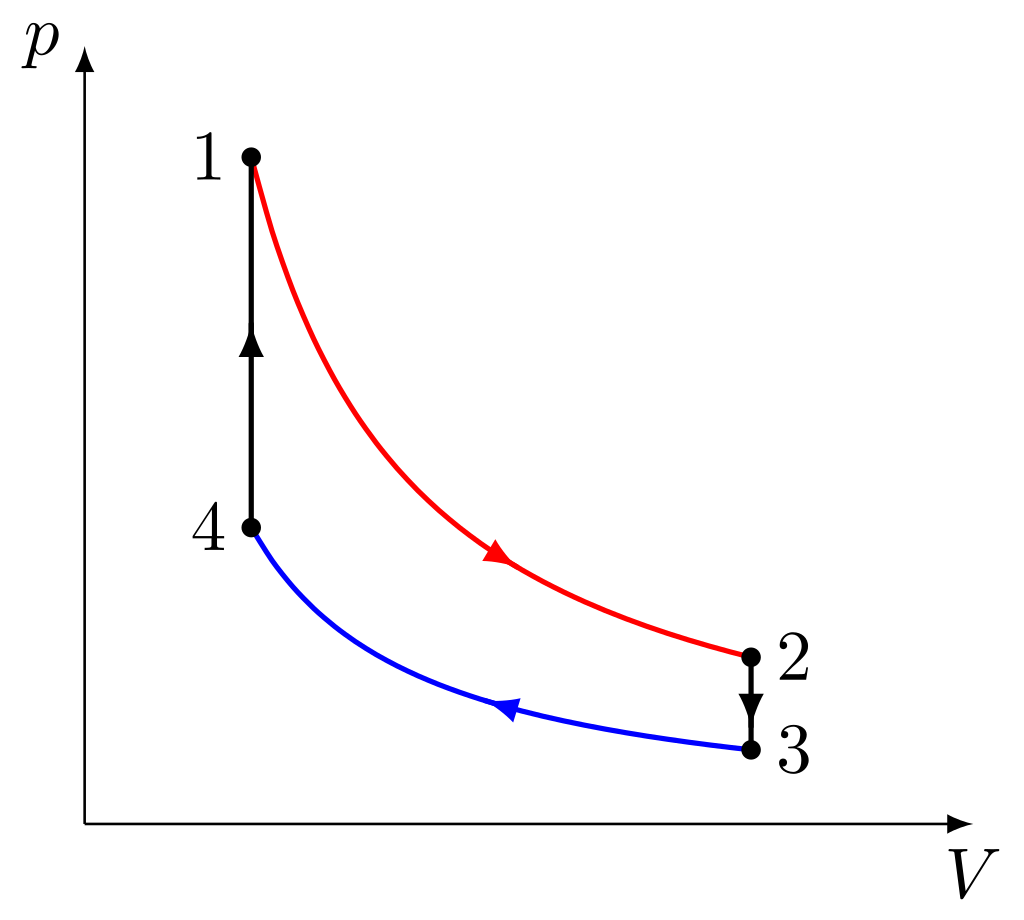
\includegraphics[scale=0.25]{Ciclo-termodinamico.png}
\caption{ciclo termondinámico}
\end{figure}

\newpage
\section{Equilibrio termodinámico:}



\subsection{Introducción: temperatura como noción empírica}
Como sabemos longitud de una varilla de hierro no solo depende de la fuerza a la que este sometido por compresión (o estiramiento) si no que también depende de la \textit{temperatura} de la propia varilla. Es decir L=L(F) no es suficiente. \\

El volumen de un gas a presión constante también depende de la \textit{temperatura} del propio gas. Entonces p=p(V) no es suficiente. \\

Entonces es evidente que existe un parámetro termodinámico desconocido que esta influyendo de manera significativa en nuestros resultados. A este parámetro lo denominaremos \textbf{temperatura empírica}, simbolizado con $ \theta $. Entonces podremos reescribir las anteriores ecuaciones de estado como P = P(X, $\theta$), llamando a \textbf{P la magnitud intensiva} y a \textbf{X la magnitud extensiva}. \\

Esta nueva magnitud es capaz de alterar el estado de un sistema por procedimientos ni mecánicos, ni electromagnéticos ni químicos. 

\subsection{Equilibrio térmico}

Si consideramos un sistema C formado por dos subsistemas simples aislados, y por lo tanto en equilibrio. Estos dos subsistemas están separados por una pared adiabática impermeable y rígida (vamos, una pared totalmente aisalada), por lo que ambos subsistemas están en equilibrio de \textit{manera individual}. Ahora cambiamos la pared y permitimos el intercambio de calor (adiabática $\longrightarrow$ diatérmica). Entonces A y B comienzan a cambiar de estado hasta que ambos están en equilibrio mutuo, cambiando solo sus propiedades intensivas (el volumen permanece igual, por lo que las extensivas son constantes). Podremos decir que ambos están en equilibrio térmico una vez \textit{satisfagan} la ecuación: $$ F(X_A, X_B, P_A', P_B')=0 $$

El equilibrio por pared diatérmica impone una ligadura sobre los valores de los subsistemas que interaccionan, es decir, \textit{se establece una relación entre ellos}, entre sus coordenadas termodinámicas, por lo que dejan de ser independientes. Para que dos sistemas estén en equilibrio térmico tienen que cumplirse dos propiedades: \begin{itemize}

\item \textbf{Reflexiva:} todo equilibrio térmico de un sistema está en equilibrio consigo mismo.

\item \textbf{Simetría:} si un sistema está en equilibrio térmico con otro este segundo debe estar en equilibrio térmico con el primero, ya que la condición de equilibrio térmico carece de \textit{direccionalidad}.

\end{itemize}

Además tiene que cumplir la condición de \textbf{transitividad}, lo que permite que el equilibrio térmico sea una relación de equivalencia. Esta condición también es conocida como la ley cero de la termodinámica. 

\subsection{Principio cero de la Termodinámica y temperatura empírica:}

\Teorema{\textbf{\underline{Principio cero de la termodinámica:}} dos sistemas termodinámicos en equilibrio térmico con un tercero están en equilibrio térmico entre sí.} \\  

Entonces debido a las condiciones de equilibrio:

$$ \begin{Bmatrix}
A \thicksim B &  \longrightarrow & f_{AB} (X_A, P_A; X_B, P_B) = 0\\
A \thicksim C & \longrightarrow & f_{AC} (X_A, P_A; X_C, P_C) = 0
\end{Bmatrix} \Longrightarrow B \thicksim C \longrightarrow f_{BC} (X_B, P_B; X_C, P_C) = 0$$

Esto se puede demostrar facilmente despejando una de las coordenadas de A de una ecuación e igualando. De hecho podemos demostrar fácilmente que al despejar queda una ecuación g dependiente de $X_A$ y de las coordenadas de B y C, pero como esta no debería aparecer asumimos que depende linealmente de las otras cuatro coordenadas de tal forma que nos aparece una relación tal que: 

$$ \theta = \theta_A (X_A, P_A) = \theta_B (X_B, P_B) = \theta_C (X_C, P_C) $$ 

A esta propiedad del estado que se iguala en el equilibrio térmico la conocemos como \textbf{temperatura empírica}. Si los sistemas están en equilibrio térmico esta variable es la misma para todas, pero no la naturaleza de ella  (es decir la \textit{función temperatura empírica}, $\theta (X,P)$,  cambia en función del sistema). Por esa razón la temperatura medida con diferentes termómetros es diferente.  \\

Una vez dicho esto pasaremos a definir a la temperatura $\theta$ como una variable, ya que como hemos podido comprobar la temperatura es una cualidad compartida por aquellos estados en equilibrio térmico, que se puede comprobar de manera macroscópica, y por lo tanto experimentalmente. Es decir $\theta=\theta(X_A, P_A)$ es una propiedad que liga las variables mecánicas con la temperatura. Ahora será una variable independiente intensiva. Otra de sus propiedades es que aquellos sistemas en equilibrio térmico tendrán la misma temperatura (cualidad común en sistemas en equilibrio térmico).

\subsection{Medida y escalas de temperatura:}

Para medir la temperatura normalmente lo que buscamos es que la temperatura quede en función de una sola magnitud mecánica, a poder ser la intensiva (haciendo que X = cte). Llamamos a P la \textbf{magnitud termométrica}:
$$ \theta = \theta (P) $$


Para conocer la temperatura de un sistema usaremos un sistema termodinámico de referencia que nos permitirá la propiedad transitiva de equivalencia \textit{estar en equilibrio térmico} de tal modo que podría ponerse en contacto con otros sistemas para medir la temperatura. El sistema de referencia llamado \textbf{termómetro} será entonces un sistema termodinámico con el cual podremos comprobar la temperatura (mediante una escala y usando las propiedades de la temperatura) de otro simplemente poniéndolos en equilibrio térmico (entonces pasarán a compartir la misma temperatura y la temperatura que facilmente podemos obtener del termómetro será la misma que la del otro sistema). \\

Una  \textbf{escala de temperaturas} es un conjunto de reglas que definen los criterios por los que es posible establecer una correspondencia biunívoca entre la propiedad temperatura y un valor numérico. Al escoger una escala de temperatura lo que se pretende es establecer una relación biunívica entre la magnitud termométrica y la temperatura. \\

La escala de temperaturas lineal permite definir la temperatura como una ecuación de grado uno respecto la magnitud termométrica:
$$ \theta = aX + b $$
Una vez tenemos la relación lo que hacemos es coger dos puntos de X ($X_1$ y $X_2$) fáciles de reproducir. A continuación lo que se hace es hallar a y b (resolver el sistema de ecuaciones) y luego substituirlo en la ecuación para un X y $\theta$ cualquiera de tal forma que:
$$ \theta = \theta_1 + (\theta_2- \theta_1)\dfrac{(X-X_1)}{(X_2-X_1)} $$. 

Por ejemplo la \textbf{escala celsius} asigna a $X_1$ la temperatura del hielo fundente tal que $\theta_1=0 ^oC$ y a $X_2$ la del vapor de agua en equilibrio con agua líquida tal que $\theta_2=100 ^oC$


\subsection{Termometría: termómetro de gas y temperatura absoluta en la escala del gas ideal}

Normalmente las determinaciones de las temperaturas se basan en la termometría de gases (ya que es una escala absoluta) pero normalmente usamos otro tipo de termómetros como, aunque el mas relevante será el de gases ideales:

\begin{itemize}
\item Termómetro de dilatación de líquidos: la variable puede ser la altura del líquido...

\item Termómetro de resistencias: basado en la variación de la resistencia eléctrica de un metal en función de la temperatura. No es lineal, es cuadrática la relación

\item Termistor: basado en la conductividad eléctrica de la temperatura.  La relación es exponencial.

\item Fenómeno termoeléctrico: depende de la fuerza electromotriz ejercida por la redistribución de cargas eléctricas. Es cúbica la relación.
\end{itemize}

Y por último tenemos el \textbf{termómetro de gas a volumen constante} el mas relevante de todos. En este caso tenemos un gas a volumen constante que introducimos en hielo fundente (y cuando estén en equilibrio se mide la magnitud termométrica, en este caso la altura del líquido b, que viene dado por la presión del gas). Luego repetimos el mismo proceso para agua hirviendo en equilibrio con su vapor. \\

  \begin{figure}[t] \centering
\includegraphics[scale=0.75]{Gas-ideal.png}
\end{figure}

Si vamos retirando el gas se obtendrán presiones cada vez mas pequeñas ($p_h > p'_h$ ...). Si repetimos la experiencia con otro gas B evidentemente obtenemos datos de presiones diferentes. Lo interesante es que cuanto mas retiramos gas los valores $\dfrac{p_v}{p_h}$ se van aproximando de tal forma que cuando llegamos al $p_h = 0$ todos los gases se comportan igual, \textit{da igual el gas}. Entonces la temperatura así definida no depende de que gas sea, si no que está definida mediante una propiedad de los gases como estado de agregación de la materia, una propiedad \textit{universal}: 

$$\dfrac{T_v}{T_h} =  \lim_{p_h \ \longrightarrow \ 0} \left( \dfrac{p_v}{p_h} \right)_v = 1,36609 $$

Entonces si fijamos una escala centígrada absoluta tal que $T_h = 273,15, T_v=373.15$, calculamos la temperatura T cualquiera al colocar en estado de equilibrio nuestro termómetro, ver la nueva presión y aplicar que:
$$ \dfrac{T}{T_h} = \lim_{p_h \ \longrightarrow \ 0} \left( \dfrac{p}{p_h} \right)_v \longrightarrow T = 273,15 \lim_{p_h \ \longrightarrow \ 0} \left( \dfrac{p}{p_h} \right)_v $$

Como la presión de una temperatura cualquiera es diferente este límite no será 1,36609... si no otro valor, lo que permitirá calcular cualquier temperatura. Sin embargo ahora el único punto fijo estándar es el punto triple del agua, que le asignaremos el valor 273,16. Ver anexo \ref{Sub:anex-punto-triple} para mas sobre el punto triple. Esta escala será llamada la escala Kelvin de temperatura. Cuando definimos como unico punto fijo el punto triple estamos haciendo un cambio lineal en la escala, de tal forma que hacemos una conversión lineal que lo deja igual, tal que:

\begin{equation}
T = 273,16 \lim_{p_3 \rightarrow 0} \parentesis{\dfrac{p}{p_3}}_v
\end{equation}

\newpage

\section{Primer principio de la termodinámica:}

\subsection{Trabajo termodinámico}

Si un sistema experimenta un desplazamiento bajo la acción de una fuerza o cambio de algún parámetro decimos que se realiza un \textbf{trabajo externo}.Este puede ser ejercido \textit{sobre} el sistema o \textit{por} el sistema. \\

Existen distintos tipos de mecanismos (modificaciones clásicas como mecánicas, tamaño del sistema... o eléctricas/magnéticas, que pueden realizar trabajo sin modificar la estructura interna del sistema) por los que se realiza un trabajo. En estos casos el trabajo externo puede expresarse como una trasferencia de energía entre un sistema y otro en función del cambio de parámetros macroscópicos, como puede ser la presión-volumen. \\

Cuando el sistema tiene una coordenada extensiva X que se modifica en un proceso infinitesimal el sistema energía y ese intercambio se expresa como: 

\begin{equation}
\D 'W \footnote{Cuando en una diferencial aparece una comilla es porque es una diferencial inexacta y no solo depende del estado inicial y final, si no del sentido recorrido}= P \D X \ \ \ [W] = m \dfrac{l^2}{t^2}
\end{equation} 

Teniendo en cuenta que: 

\begin{itemize}
\item \textbf{P}: fuerza generalizada
\item \textbf{X}: desplazamiento generalizado
\end{itemize}

Tanto el desplazamiento generalizado como la fuerza generalizada se llamaran variables mecánicas. Siempre aparecen por pares, como pueden ser presión-volumen, fem-carga, fuerza-longitud... Una variable extensiva siempre conllevará su magnitud intensiva conjugada. \\

El trabajo puede realizarse sobre el sistema o ser realizado por el sistema. En termodinámica tendremos en cuenta para el criterio de signo la coincidencia de que la fuerza externa que actúa sobre el sistema tenga el mismo sentido que el desplazamiento. Si coinciden \textit{se realiza trabajo sobre el sistema} y es positivo. Si la fuerza externa ejercida es contraria al desplazamiento es negativo, y el \textit{el trabajo es realizado por el sistema}. \\

\begin{figure}[h!] \centering
\includegraphics[scale=0.5]{trabajo termodinamico.png}
\caption{trabajo realizado sobre/por el sistema}
\end{figure}



\subsection{Coeficientes térmicos}

Se van a definir cuatro coeficientes termodinámicos que expresan las variaciones relativas de T, P y X: 

\begin{itemize}
\item \textbf{Coeficiente de dilatación térmico:} varía la coordenada extensiva respecto la temperatura con la coordenada intensiva constante:

\begin{equation}
\alpha = \dfrac{1}{X} \left( \dfrac{\partial X}{\partial T}\right)_{P}
\end{equation}

\item \textbf{Coeficiente piezométrico:} varía la coordenada intensiva respecto la temperatura a la coordenada extensiva constante (por eso X abajo):

\begin{equation}
\gamma = \dfrac{1}{P} \parentesis{\dfrac{\partial P}{\partial T}}_{X \footnote{Significa que la variación es a magnitud extensiva constante)}}
\end{equation}

\item \textbf{Coeficiente de compresibilidad isotérmico:} nos indica como varía la coordenada extensiva respecto la intensiva a temperatura constante:

\begin{equation}
k_T = \dfrac{1}{X} \parentesis{\dfrac{\partial X}{\partial P}}_T
\end{equation}

\item \textbf{Coeficiente de comprensibilidad adiabático:} nos indica como varía la  coordenada extensiva respecto la intensiva a entropía constante:

\begin{equation}
k_s = \dfrac{1}{X} \parentesis{\dfrac{\partial X}{\partial P}}_S
\end{equation}

\end{itemize}

Si tenemos una ecuación de tres variables tal que $\phi(x,y,z) = k$ siendo k una constante se verifica que::

\begin{equation}
\parentesis{\frac{\partial x}{\partial y}}_z \parentesis{\frac{\partial y}{\partial z}}_x \parentesis{\frac{\partial z}{\partial x}}_y = -1
\end{equation}

Entonces si estás variables son P, X y T tenemos que podemos usar esto, de tal forma que substituyendo por los distintos coeficientes (y haciendo alguna inversa) tenemos que: 

\begin{equation}
\alpha = - P \gamma k_T
\end{equation}

\subsection{Primer principio de la termodinámica}
El primer principio de la termodinámica nos dice que en un proceso en el que solo se intercambie energía, da igual la forma en la que se intercambie, siempre que se intercambie la misma cantidad de energía desde el mismo estado inicial el sistema termodinámico tendrá el mismo estado final. Es decir, que si aportamos cierta cantidad de energía mediante un trabajo mecánico, el estado final del sistema será el mismo que si aportamos esa misma cantidad de energía de forma calorífica. Entonces tiene que haber una función de estado que lo que nos diga es que da igual la forma en la que aportes la energía ese estado va a cambiar hacia el mismo equilibrio. Esta nueva función de estado es conocida como \textbf{energía interna (U)} (es función de estado ya que solo importa el estado inicial y final, da igual el recorrido). En general será imposible conocer la cantidad concreta de energía interna de un sistema con un estado termodinámico dado, ya que depende de la cantidad de energía que podamos extraer del sistema. Sin embargo la diferencia de energía interna entre dos estados de equilibrio si es algo que podamos conocer porque la diferencia energía interna es igual que la energía que ha intercambiado con el sistema. Como la energía que se puede intercambiar puede ser \textbf{trabajo} o \textbf{calor}:

$$  \Delta U   = U_2 - U_1 = Q_{12} + W_{12}$$
\\ 

Aunque estemos mencionando ya la energía interna y el calor todavía no hemos definido estos conceptos formalmente, lo que haremos tras formular el primer principio de la termodinámica. \\

\Nota { puede caer en el examen tanto la definición clásica del primer principio de la termodinámica como enunciados mas modernos. } \\ \\


La \textbf{formulación clásica} del primer principio de la termodinámica no viene definido por la energía interna ni por el calor, si no por el simple enunciado de que es imposible construir un dispositivo que funcionando por ciclos (\ref{def:ciclo}) realice constantemente trabajo sobre el entorno sin que absorba ningún tipo de calor del entorno. Es decir, la formulación clásica del primer principio de la termodinámica afirma la \textit{imposibilidad del móvil perpetuo de primera especie}. Es un problema que este enunciado presuponga que conocemos el concepto de calor, ya que todavía no lo hemos definido formalmente, aunque podamos comprender que es \\

Con la \textbf{formulación de Born} del primer principio ya se nos introduce el concepto de energía interna. Sin embargo la energía interna viene definida, al menos en un principio, por medios puramente mecánicos. Como ya sabemos en un proceso adiabático el sistema solo puede intercambiar energía con el entorno mediante el trabajo. Entonces si tenemos un sistema cerrado asilado adiabáticamente, si hacemos cambiar al sistema desde un estado 1 a un estado 2 mediante trabajo mecánico tenemos que la cantidad de trabajo necesaria para este cambio sólo depende del trabajo efectuado y no de los medios mediante los cuales se realiza el proceso, no depende de las etapas intermedias. Entonces ya tenemos lo necesario para formular nuestro primer principio de la termodinámica, ya que nuestra nueva forma de entender el primer principio no depende ni de la energía interna:  \\


\Teorema{\textbf{\underline{Primer principio de la termodinámica}}: el primer principio de la termodinámica nos dice que el trabajo realizado sobre un sistema adiabáticamente aislado depende, exclusivamente, de los estados inicial y final. En general se escribe:
$$ \Delta U = W^{adib} \Longrightarrow  $$
$$ \D U = \D ' W +  \D ' Q \Longleftrightarrow \Delta U = W + Q $$
} \\ \\

Entonces si conideramos $\{ x_i \}$ las coordenadas termodinámicas que definen cualquier estado, teniendo en cuenta que $x_1$ define un estado 1, $x_2$ un estado 2 y $x_3$ un estado 3. Ahora supongamos que viaja del estado 1 al estado 2 mediante un trabajo adiabático. Entonces, teniendo en cuenta el primer principio tenemos que: 

$$ W_{12}^{adib} = F(\lbrace x_1 \rbrace , \lbrace x_2 \rbrace);  W_{23}^{adib} = F(\lbrace x_2 \rbrace , \lbrace x_3 \rbrace) $$

Y que por lo tanto si consideramos un proceso adiabático que vaya directamente de 1 a 3 y lo comparamos con el recorrido de 1 a 2 y de 2 a 3, como el trabajo solo depende del estado final y estado inicial:

$$  W_{13}^{adib} = F(\lbrace x_1 \rbrace , \lbrace x_3 \rbrace) = F(\lbrace x_1 \rbrace , \lbrace x_2 \rbrace) + F(\lbrace x_2 \rbrace , \lbrace x_3 \rbrace)$$

Y para que esto se verifique en todo momento, da igual el estado inicial y final y cuantos caminos hayamos recorrido, es una condición necesaria que se cumpla que:  $  = F(\lbrace x_1 \rbrace , \lbrace x_2 \rbrace) = U{x_2}-U{x_1}$... \\

Entones ahora podemos definir formalmente la \textbf{energía interna} como una propiedad tal que la diferencia entre sus valores en el estado final e inicial es igual al trabajo total realizado sobre el sistema a lo largo de cualquier proceso adiabático que una los estados de equilibrio 1 y 2. De esta forma queda definida mediante procesos puramente mecánicos (los adiabáticos). Matemáticamente: \\


\begin{equation}
\Delta U_{12} = W_{12}^{adib}
\end{equation}



\subsection{Definición de calor}

Supongamos que vamos de un estado 1 a un estado 2 mediante un proceso adiabático, de tal manera que $\Delta U = W_{12}^{adib}$. Ahora supongamos que pasamos del estado 1 al estado 2 mediante un proceso no adiabático, realizando un trabajo $W_{12}$. Entonces está claro que $W_{12} \neq W_{12}^{adib}$. Si el proceso sigue trasformando el sistema del estado 1 al estado 2, y la diferencia de energía interna es la misma, pero el trabajo por los dos caminos no es el mismo. ¿Como podemos explicar el proceso no adiabático? Pues hay algún tipo de trasferencia energética que no implique el trabajo que no estamos teniendo en cuenta. A esta trasferencia energética llamamos \textbf{calor (Q)}. \\

Por consecuencia la diferencia enerética entre el trabajo por un proceso adiabático y el trabajo por un proceso no adiabático será el calor intercambiado por el sistema en el proceso no adiabático:

\begin{equation}
Q_{12} = W_{12}^{adiab} - W_{12} \Longrightarrow \Delta U_{12}=W_{12}^{adiab}=Q_{12}+W_{12} 
\end{equation}

Para un proceso infinitesimal: $$ \D U = \D ' W `+ \D ' Q $$


\subsection{Calor específico}

Experimentalmente se observa que cada cuerpo necesita un aporte de calor diferente de otro para elevar su temperatura cierta magnitud. Por ejemplo, es mas difícil calentar un gramo de agua que un gramo de aluminio, necesitamos mucho menos calor. Para caracterizar esta propiedad creamos el \textbf{calor específico} o \textbf{capacidad calorífica}. Aunque lo endentemos de forma general como el calor que hace falta aportar para que aumente una temperatura $\Delta T$, realmente la definición anterior se puede precisar en el caso de un proceso infenitesimal: 

\begin{equation}
C_{\gamma} = \parentesis{\dfrac{\D ' Q}{\D T}}_{\gamma} = \parentesis{\dfrac{\partial Q}{\partial T}}_{\gamma}
\end{equation}

La $\gamma$ es la variable termodinámica que permanece constante en el proceso de suministro de calor. Puede ser, por ejemplo, la variable extensiva X, o la intensiva P. También nos podemos encontrar la \textbf{capacidad calorífica molar} que es la capacidad calorífica respecto el número de moles: 

\begin{equation}
c_{\gamma} = \dfrac{1}{n} \parentesis{\dfrac{\D ' Q}{\D T}}_{\gamma}
\end{equation}

\newpage
\section{Segundo principio de la termodinámica:}
\subsection{Limitaciones del Primer Principio:}
El primer principio insiste en a validez del principio general de la conservación de la energía, definiendo para ello la energía interna, o mas bien la diferencia de energía interna de un sistema: 

$$ \D U = \D ' Q + \D ' W $$

Ahora bien, ¿Son viables todos los procesos en los que se conserva la energía? La respuesta rápida es que no, no es posible. En experimentos ideales se puede convertir toda la energía de un tipo en energía de otro tipo y viceversa, pero en la realidad existen perdidas de energía inevitables que provocan una \textit{irreversibilidad}: no toda la energía en forma de calor puede transformarse en otra clase de energía. En la naturaleza muchas veces los procesos ocurren en un sentido de manera espontánea pero el sentido opuesto no ocurrirá de manera espontánea. Por ejemplo si tenemos dos sistemas aislados A y B a diferente temperatura $T_1$ y $T_2$. Si ahora permitimos el contacto térmico entre ambos sistemas las temperaturas evolucionarán hasta que estén en equilibrio termodinámico, evolucionando a una temperatura $T_3$. Si volvemos a aislar los sistemas, las temperaturas de A y B no volverán a ser $T_1$ y $T_2$ de manera espontánea. \\

El \textbf{segundo principio} de la termodinámica tratará esto: la imposibilidad de utilizar la energía de forma particular, y en que sentido se produce un proceso de forma espontánea. Es totalmente independiente del primer principio. 


\subsection{Máquinas térmicas y máquinas frigoríficas}
Sea un proceso cíclico cualesquiera: 
\begin{equation}
\oint \D U  = \oint \D ' W + \oint \D ' Q \Longrightarrow  \oint \D ' W = - \oint \D ' Q  \Longrightarrow W = -Q
\end{equation}
Un cíclico es un proceso en el que el estado inicial y final es el mismo (ej: A $\rightarrow$ B $\rightarrow$ C $\rightarrow$ A), siendo A B y C estados termodinámicos. Normalmente usamos los procesos cíclicos ya que nos  permite encontrar la cantidad de calor intercambiado refiriéndolas al trabajo. Cuando hablamos de procesos cíclicos en general hablaremos de aquellos procesos que impliquen \textbf{máquinas térmicas}, que es realmente donde podemos encontrar de manera práctica estos procesos. Para entender primero las máquinas térmicas tenemos que introducir los siguientes conceptos:

\begin{itemize} 
\item \textbf{Sustancia de trabajo:} es nuestro sistema termodinámico (gas, líquido... que realiza el ciclo termodinámico). Ej: gas de la nevera.

\item \textbf{Fuente (foco) de calor:} sistema físico generalmente en contacto con la sustancia que proporciona o absorbe energía de calor sin que se modifique ni la temperatura ni cualquier otra de sus coordenadas termodinámicas. 

\item \textbf{Máquina o motor térmico:} cualquier mecanismo que contenga al sistema y que le obligue a seguir un ciclo, es decir, cualquier sistema termodinámico que produzca trabajo o calor consumiendo una cantidad de calor o trabajo. Ej: motor de un coche.
\end{itemize}

Una vez entendemos esto podemos hablar de las máquinas térmicas, que son:

 \begin{itemize}
 
\item \textbf{Motores:} en los motores existe un proceso durante el cuál se produce absorción de calor de una fuente externa de alta temperatura (foco caliente), de tal modo que es capaz con el calor absorbido suministrar trabajo al exterior así como ceder parte del calor a un foco frío. \\
  
\begin{figure}[h!] \centering
\includegraphics[scale=0.6]{Máquina-termica.png}
\end{figure} 


\item \textbf{Frigoríficos:} en este caso la máquina térmica cede calor a sustancia de trabajo, y aplicandole un trabajo a esta conseguiremos pasar calor a la fuente de calor. En una nevera la sustancia de trabajo es el gas, la electricidad el trabajo mecánico que se aporta.  

\begin{figure}[h!] \centering
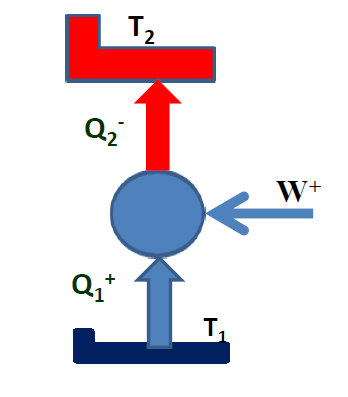
\includegraphics[scale=0.6]{Máquina-frigorífica.png}
\label{fig:4-maquina-frigorifica}
\end{figure}

\item \textbf{Bomba de calor:} una bomba de calor es una máquina térmica que puede actuar como calentador y como refrigerador en función de lo que queramos. Un ejemplo sería aire acondicionado, que puedes hacer que caliente o enfríe tu habitación.

\end{itemize} 

\subsection{Enunciados clásicos del Segundo Principio}

Existen dos postulados del 2º principio, que mediante el uso de máquinas térmicas y ciclos nos establecen la imposibilidad de algunos procesos. Ambas se complementan, y una implica la otra (aunque eso lo demostraremos mas tarde). Los postulados son \\:

\Teorema{\textbf{\underline{Postulado de Kelvin-Plank (K-P)}}: no es posible ningún proceso cuyo único resultado sea la absorción de calor procedente de un único foco y su conversión íntegra en trabajo (imposibilidad del móvil de segunda especie). } \\ \\

\Teorema{\textbf{\underline{Postualdo de Clausius (CL)}}: no es posible ningún proceso cuyo único resultado sea la trasferencia de calor de un cuerpo a otro que se encuentre a temperatura superior. } \\ \\


\begin{figure}[h!]
\centering
\includegraphics[scale=1]{clausius.png}
\end{figure}

Ahora demostramos la relación entre ambos postulados:

\begin{itemize}
\item CL $\longrightarrow$ K-P: si negamos el postulado de clausius, es decir, existe el refrigerador perfecto, podemos construír una máquina tal que tenga un refrigerador perfecto intercambiando calor del foco frío ($Q_1^+$) al foco caliente ($Q_2^-$), y otra máquina que absorba calor del foco caliente ($Q_2 '^+$) y trasforme este calor en trabajo al medio externo ($W^-$) y que trasfiera un poco de ese calor al foco frío ($Q_1'^-$). 

\begin{figure}[h!]
\centering 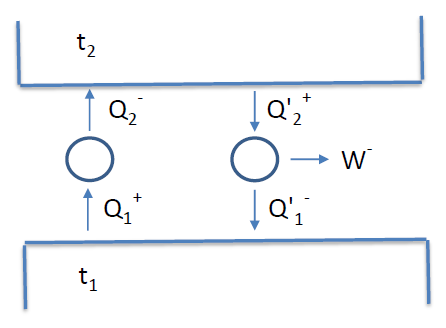
\includegraphics[scale=0.5]{CL-KP.png}
\end{figure}

Tenemos que $Q_1^+ + Q_1'^- = 0$ (imponemos esta condición para que el foco no se caliente, además que de otro modo el experimento no tendría sentido), y que $Q_1^+ + Q_2^-=0$. Entonces como $Q_1'^- + Q_2'^+ + W^- = 0$ (recordemos que las máquinas trabajan por ciclos), tenemos que:

$$ Q_2^- + Q_2'^ + W^- = 0 \Longrightarrow Q_2^- + Q_2'^+ = Q_{T2}^+ > 0 \Longrightarrow Q_{T2}^+  + W^- = 0  $$

Es decir al negar el enunciado de Clausius hemos demostrado que también negamos el enunciado de Kelvin-Planck, ya que exista una máquina que realmente trasforme todo el calor que recibe en trabajo.  Como el foco frío no cambia de energía interna ni el refrigerador perfecto podemos perfectamente ``omitirlos'' de tal forma que solo quede el motor térmico perfecto. 


\item K-P $\longrightarrow$ CL: si negamos el postulado de Kelvin-Plank (por lo tanto afirmamos que existe la máquina térmica perfecta) llegaremos a la conclusión de que también existirá el refrigerador perfecto. Supongamos entonces el siguiente esquema: 


\begin{figure}[h!]
\centering 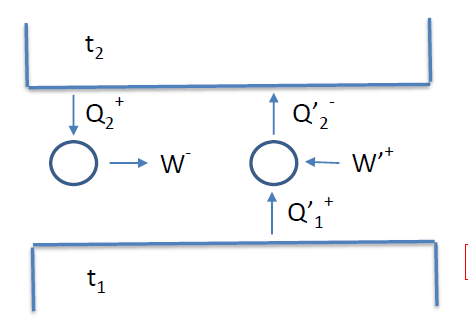
\includegraphics[scale=0.5]{KP-CL.png}
\end{figure}


Entonces tenemos que el la máquina térmica perfecta ejerce un trabajo que inmediatamente suministra al refrigerador perfecto de tal manera que $W'^+ + W^- = 0$. Entonces como el la máquina térmica extrae la misma cantidad de calor que ejerce trabajo: $Q_2^+=-W^-$. Además el refrigerador cumple que $W^+ + Q_1'^+ + Q_2'^-=0$. Substituyendo todo esto tenemos que:

$$ Q_2^+ + Q_2'^- + Q_1'+ = 0 $$

Por lo tanto tenemos que $Q_2^+ <Q_2^-$ entonces si $Q_{T2}^- = Q_2^+ + Q_2^- < 0$. Entonces podemos extraer una cantidad de calor $Q_1^+$ del foco caliente y ceder $Q_{2T}^-$ a otro foco $t_2$ sin necesidad de aportar trabajo, demostrando lo que queríamos demostrar.


\end{itemize} 

Hemos llegado a la conclusión de que si se afirma un postulado se afirma el otro y viceversa. \\

\Nota{en general los superíndices + y - indican que el calor o trabajo es positivo (es decir absorbido/realizado sobre el sistema) o negativo (emitido/realizado por el sistema).} \\ \\


\Nota{puede caer en el examen las definiciones del segundo postulado de Kelvin-Planck y Clausius, así como su relación. }

\subsection{Rendimiento y eficiencia}
El rendimiento de una máquina viene dado en función de cual sea su ciclo, pero siempre nos aporta una medida de cuan está cerca de ser perfecta esa máquina. Entonces tenemos que: 

\begin{itemize}
\item \textbf{Máquina térmica:} el rendimiento de una máquina térmica (siendo $Q_2$ el calor absorbido del foco caliente, W el trabajo realizado por la máquina y $Q_1$ el calor absorbido por el foco frío) será:

\begin{equation}
\eta = - \frac{W^-}{Q_2^+} = \frac{Q_2^+ + Q_1^-}{Q_2^+} = 1 + \dfrac{Q_1^-}{Q_2^+} = 1 - \dfrac{Q_1^+}{Q_2^+} \label{eq:4-rendimiento-maquina-termica}
\end{equation}

El rendimiento máximo e inalcanzble será por lo tanto $\eta = 1$. Está sería la máquina de kelvin-plank. \\


\item \textbf{Máquina frigorífica:} el rendimiento en un frigorífico es prácticamente igual, solo hay que tener en cuenta que el ``refrigerador perfecto'' (máquina de Clausius) es aquel que es capaz de enfriar el foco frío recibiendo la menor cantidad de trabajo posible:

\begin{equation}
\eta = \varepsilon = \dfrac{Q_1^+}{W^+}  = \dfrac{Q_1^+}{Q_2^+ + Q_1^-}
\label{Ec:4-rendimiento-frigorifico}
\end{equation}

En este caso el rendimiento límite sería $\eta = \infty$, no puediendo llegar al infinito porque tendríamos una máquina de clausius, ya que siempre tenemos que aportar un trabajo. Al rendimiento en este caso también lo llamamos \textbf{eficiencia ($\varepsilon$)}. \\



\item \textbf{Bomba de calor:} en función de si actúa como calentador o como refrigerador tenemos distintas maneras de evaluar el rendimiento. Si actúa como calentador:

\begin{equation}
\eta = \varepsilon = - \dfrac{Q_2^-}{W^+}
\end{equation}

Siendo $W^+$ el trabajo que aporta el medio externo, y $Q_2^-$ el calor que intercambia con el foco caliente, tal y como en la figura \ref{fig:4-maquina-frigorifica}. En este caso el rendimiento máximo será 1, ya que si todo el trabajo que se recibe se transforma en calor tendremos la bomba de calor perfecta. En el caso del refrigerador el rendimiento será el mismo que en la ecuación \ref{Ec:4-rendimiento-frigorifico}. Al igual que antes también llamamos al rendimiento \textbf{eficiencia}.
 
\end{itemize}
 

\subsection{Ciclo de Carnot}

El ciclo de carnot es un proceso cíclico en el que nuestra substancia de trajo intercambia trabajo y calor entre un foco frío ($T_1$) y un foco caliente ($T_2$). El intercambio de calor se produce mediante procesos reversibles, de tal modo que la  trasferencia de calor no aumente la temperatura. En el caso de aumentar la temperatura el proceso no podría ser reversible, ya que sería imposible volver al estado anterior (si la máquina pero no el entorno). Los procesos de calentamiento y enfriamiento para que sean reversibles deben ocurrir para Q=0, de tal forma que estos procesos sean adiabáticos. \\

Entonces de forma general definimos un \textbf{ciclo de carnot} como un ciclo donde hay 2 procesos isotérmicos y 2 procesos adiabáticos de tal manera que es reversible:

\begin{figure}[h!]
\centering
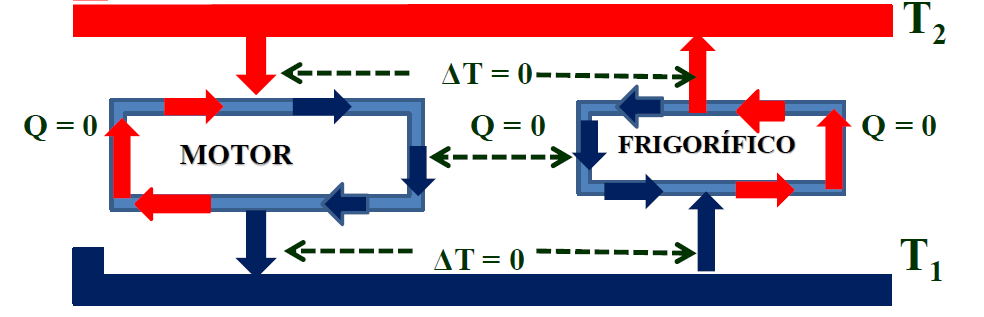
\includegraphics[scale=0.4]{Ciclo-de-carnot.png}
\end{figure}

Como podemos ver en las figura \ref{fig:4-ciclo-carnot1} tenemos que la el trabajo ejercido por la máquina térmica es positivo, y para compensar el calor debe ser negativo. Es decir, mientras el gas (consideremos que es un gas aunque es válido para cualquier material) ejerce trabajo sobre el medio externo al ($W<0$) como hemos visto el calor debe ser absorbido de foco caliente, y aunque expulse calor ($Q_2<0$) el total es positivo. Esto se ve de manera cualitativa observando las areas, pero también se puede ver de manera cuantitativa. Si fuera un gas ideal sería muy fácil de deducir simplemente viendo que $W_T<0$ y por ser un ciclo $\Delta U = 0$ entonces $Q_T>0$. Además es evidente que  $\eta \neq 100\% $ ($Q_2^+ > -W_T$ ya que expulsa calor ($Q_1^-<0$)). \\

\begin{figure}[h!] \centering
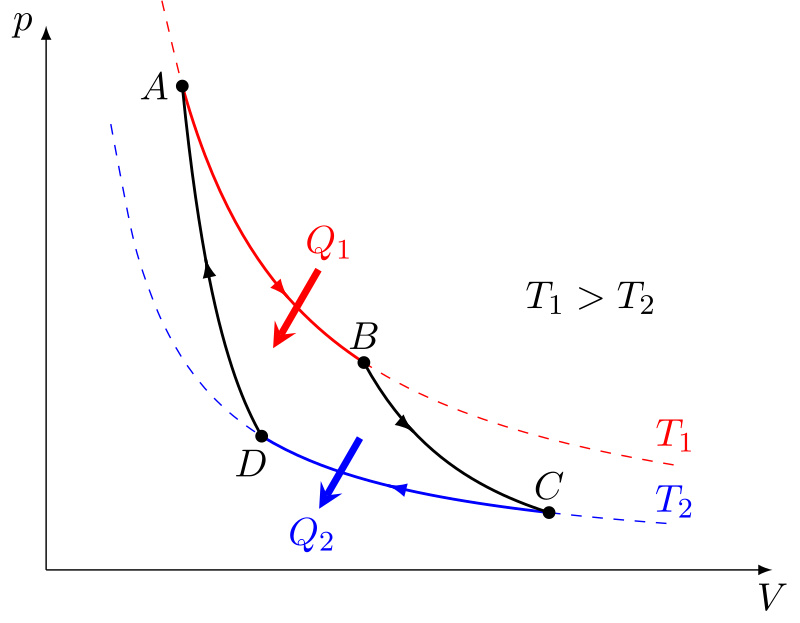
\includegraphics[scale=0.3]{Ciclo-de-carnot-1.png}
\caption{ciclo de carnot para una motor térmico}
\label{fig:4-ciclo-carnot1}
\end{figure}



Con esto lo que quiero demostrar es que es un ciclo de carnot que no viola ningún principio de la termodinámica visto hasta ahora, y por lo tanto el ciclo existe. 

\subsection{Teorema de Carnot}

El teorema de Carnot es un enunciado alternativo del Segundo Principio de la Termodinámica que se formula a partir de la comparación de entre máquinas irreversibles y reversibles. Este teorema nos dice que: \\

\Teorema{\textbf{\underline{Teorema de Carnot}:} de todas las máquinas térmicas aquella que funciona de forma reversible es la que tiene el mayor rendimiento. Además dos máquinas reversibles que operen entre los mismos focos tendrán el mismo rendimiento. Otra forma de verlo sería: sea M una máquina térmica cualquiera que opera entre dos focos térmicos y sea C la máquina térmica reversible que opera entre los mismos focos. Entonces: $$ \eta_M \leq \eta_C $$ Verificándose la igualdad cuando M también es máquina térmica reversible.} \\ \\

Entonces lo que trataremos de demostrar es que en primer lugar de dos máquinas térmicas trabajando entre los mismos focos la que funciona de forma reversible es la que tiene mayor rendimiento, y luego veremos que todas las reversibles tienen el mismo rendimiento. \\

Supongamos un esquema como el de la \ref{fig:4-teorema-carnot}. En la izquierda tendremos una máquina reversible que funciona mediante ciclos de carnot (izquierda) y a la derecha una máquina cualquiera. Como es reversible podemos invertir su funcionamiento (y pasar de ser maquina térmica a frigorífica y viceversa). Ahora hagamos unas suposiciones. Está claro que los dos trabajos $W_R$ y $W$ serán iguales. Esto lo hacemos para estudiar mejor el rendimiento de la máquina, ya que la diferencia entre ambos rendimientos ahora solo dependerá del calor que ambos absorban. Para la figura de la izquierda podemos obtener lo siguiente:


\begin{equation}
\left. \begin{array}{ll}
Q_{2R}^- + W_R^+ + Q_{1R}^+ & = 0\\
Q_2^+ + W^- + Q_1^+ & = 0\\
\end{array} \right\rbrace \Longrightarrow Q_{2R}^-+Q_{1R}^++Q_2^++Q_1^- = 0
\end{equation}

Para la disposición de la izquierda:

\begin{displaymath}
\left. \begin{array}{ll}
Q_{2R}^- + Q_2^+ & \geq 0 \\
Q_{1R}^+ + Q_1^-  & \leq 0
\end{array} \right\rbrace \Longrightarrow 
\left\lbrace \begin{array}{lll}
Q_{2R}^- & \geq & Q_2^- \\
Q_{1R}^+ & \leq & Q_1^+ 
\end{array} \right.
\end{displaymath}

Y como los rendimientos vienen dados por \ref{eq:4-rendimiento-maquina-termica} entonces podemos extraer que los rendimientos:

$$ \eta_R = - \dfrac{W_R^-}{Q_{2R}^+}; \ \eta= -\dfrac{W^-}{Q_{2}^+} \Longrightarrow \dfrac{\eta_R}{\eta} = \dfrac{Q_2^+}{Q_{2R}^+} \geq 1 \Longrightarrow \eta_R \geq \eta  $$


\begin{figure}[h!] \centering
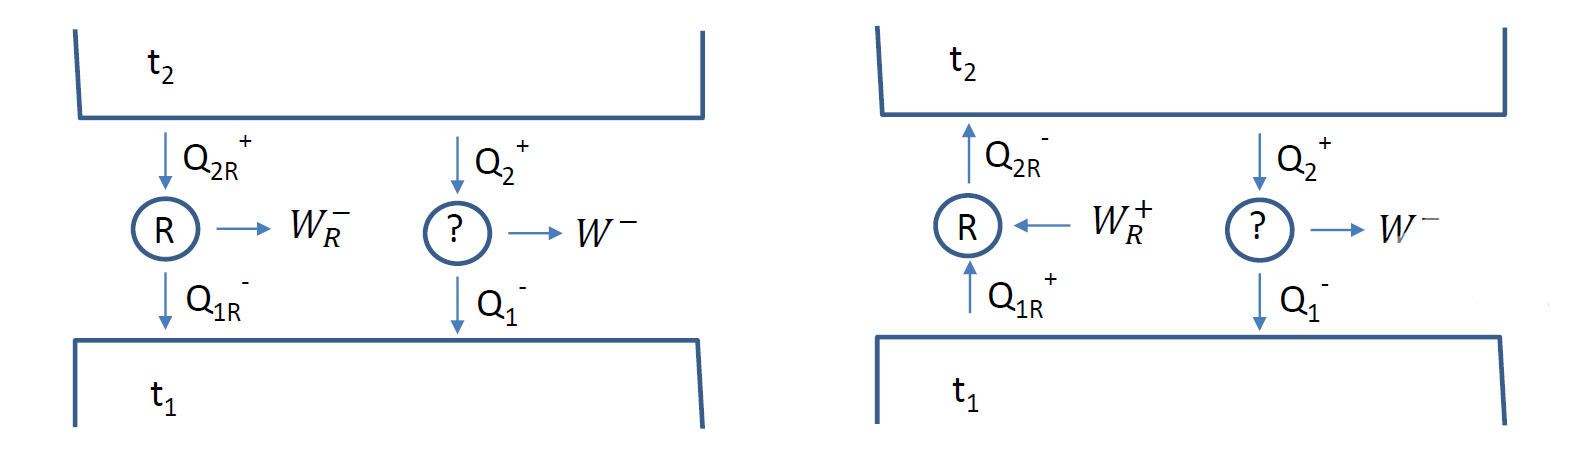
\includegraphics[scale=0.6]{Teorema-carnot.png}
\label{fig:4-teorema-carnot}
\caption{esquema de máquinas térmicas para demostrar el teorema de carnot}
\end{figure}

Por lo tanto hemos demostrado el teorema de carnot. Para que se cumpla la igualdad está claro que el calor que extraemos del foco caliente por parte de ambos tiene que ser igual. Esto solo ocurre si la otra máquina térmica también actúa mediante ciclos de carnot (ciclos reversibles). Para demostrar esto podemos suponer que actúa con otro ciclo de carnot, y podemos comprobar que en este caso se cumplirá que $Q_{2R}^+ \leq Q_2^+$ y $Q_{2R}^+ \geq Q_2^+$ por lo que tiene que suceder que $Q_{2R}^+ = Q_2^+$ y por lo tanto los rendimientos iguales. \\

Una vez demostrado esto queda claro entonces que siempre que una máquina actúe por ciclos reversibles o de carnot tendrá el mismo rendimiento no importa la sustancia de trabajo. Esto solo sucede si el rendimiento solo depende de la temperatura de los focos, de tal manera que:

\begin{equation}
\eta = 1 - \dfrac{Q_1}{Q_2} = f(T_1,T_2) \Longrightarrow \dfrac{Q_1}{Q_2} = f(T_1,T_2)
\end{equation}



\subsection{Escala termodinámica de temperatura:}

Lord Kelvin demostró que el teorema de Carnot puede emplearse para definir la escala termodinámica de temperaturas. Para demostrar esto suponemos que existe un foco intermedio a temperatura $T_3$, como se muestra en la siguiente figura:

\begin{figure}[h!] \centering
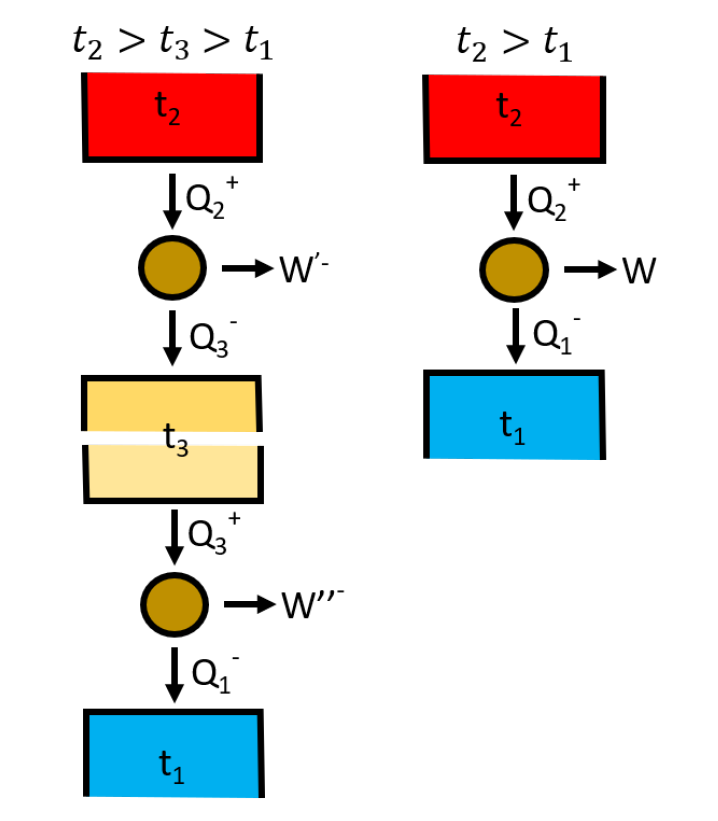
\includegraphics[scale=0.6]{Temperatura-absoluta-carnot.png}
\caption{esquema disposición máquinas térmicas. Derecha: máquina térmica equivalente.}
\label{fig:4-escala-termodinamica-temperaturas}
\end{figure}

También sabemos que en el caso de que las máquinas térmicas actúen con ciclos  de carnot el rendimiento solo dependerá de la temperatura de los focos, por lo que podemos escribir: 

$$ f(T_1,T_2) = \dfrac{Q_1}{Q_2} = \dfrac{Q_1}{Q_3} \dfrac{Q_3}{Q_2} = f_1(T_1,T_3) f_2 (T_2,T_3)  $$

Está claro que $f_1$ y $f_2$ son las funciones que relacionan los calores para cada una de las máquinas térmicas de la izquierda. Entonces si lo que buscamos es una equivalencia entre $f$ y $f_1  $ y $f_2$ está claro que en la multiplicación se deben cancelar las temperaturas $T_3$. Para que esto ocurra las funciones deben ser del tipo: 

$$ f(T_1,T_2) = \dfrac{\phi(T_1)}{\phi(T_2)} $$

De tal manera que las $\phi(T_3)$ se cancelen. Como $\phi$ es una función genérica en realidad existen infinitas posibilidades  como exponencial, logarítimica... Lord Kelvin definió la \textbf{escala absoluta o escala termodinámica de temperatura} a la función lineal $\phi (T) = CT$ donde C es un escalar (factor de proporcionalidad). \\

De hecho fue Lord Kelvin quien propuso utilizar las máquinas térmicas como termómetros, aunque al principio uso una función exponencial para hacerlo. Para eso se toma como valor de referencia el punto triple del agua (273,16 K). Entonces:

\begin{equation}
T = 273,16 \dfrac{Q}{Q_3}
\end{equation} 

Entonces por está definición $T>0$ siempre, ya que si $T \rightarrow 0$ entonces $Q^+ \rightarrow 0$, pero esto implicaría que existiría la máquina de Kelvin-Plank, lo cual viola el segundo principio. Por lo tanto es imposible que $T=0$. Entonces para las máquinas reversibles el rendimiento del ciclo de Carnot:

$$ \eta = 1 - \dfrac{Q_1^+}{Q_2^+} = 1 - \frac{T_1}{T_2}$$

Siempre que la temperatura esté definida en una escala lineal como la escala absoluta. 

\newpage

\section{Entropía}
\subsection{Teorema de Clausius: definición de entropía}


Primero vamos a suponer algunas hipótesis. Consideremos un sistema que evoluciona según un ciclo cualquiera (ciclo azul en la imagen \ref{fig:5-1}). A continuación hagamos el intento de sustituir el ciclo de otros en forma de ciclos de Carnot:

\begin{figure}[h!] \centering
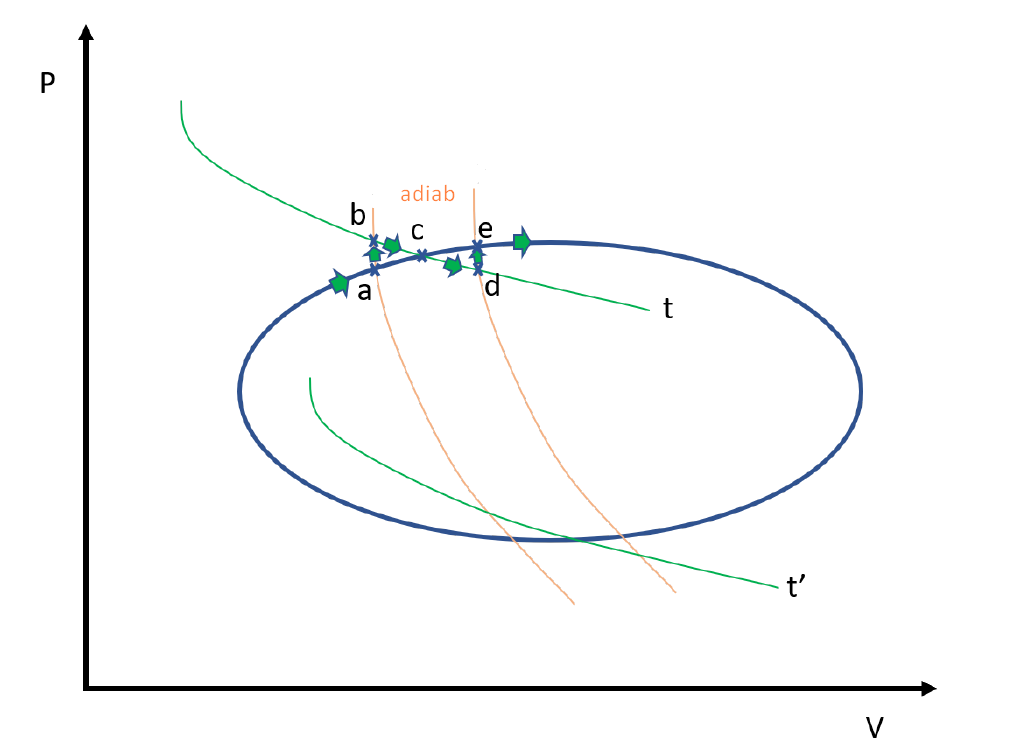
\includegraphics[scale=0.5]{teorema-clausius-1.png}
\caption{ciclo cualquiera al que se aproxima entre dos puntos por un ciclo de carnot}
\label{fig:5-1}
\end{figure}

Si nos acercamos bien a la región esa para ver que está sucediendo tenemos que:

\begin{figure}[h!] \centering
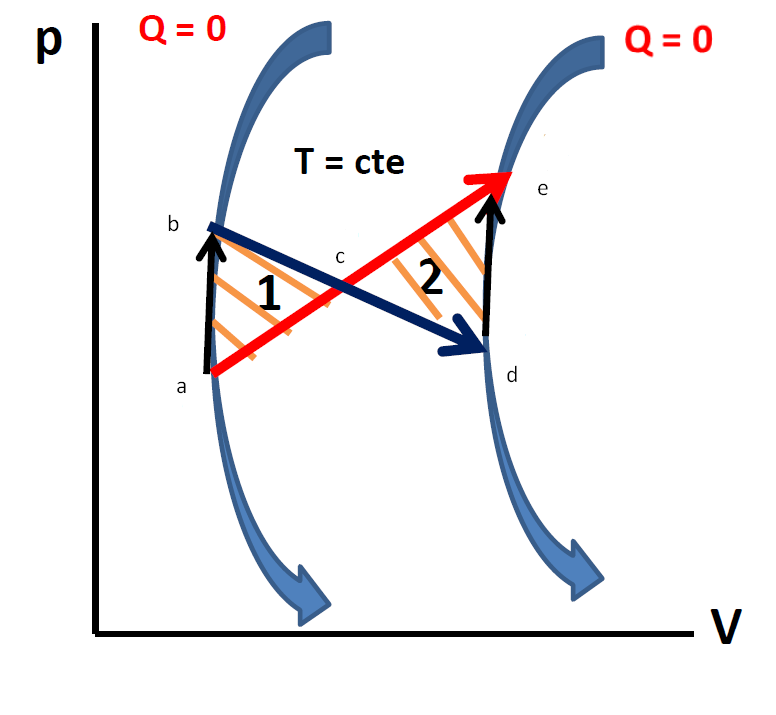
\includegraphics[scale=0.5]{teorema-clausius-2.png}
\caption{aproximación por carnot entre dos puntos del ciclo}
\label{fig:5-2}
\end{figure}

Probablemente os estaréis preguntando que está pasando aquí, por qué estamos haciendo esto. Pues bien, si nos fijamos bien en los dos procesos tenemos que uno va de a hasta e directamente, que será el \textbf{proceso a-e}; y tenemos uno que hace a-b-c-d-e, que será el \textbf{proeso a-b-c-d-e}. En ambos procesos la variación de energía interna será la misma (ya que es función de estado). Además el trabajo intercambiado entre ambos procesos será el mismo, no porque \textit{necesariamente} tenga que ser así, si no porque nosotros \textit{impondremos} que esto es así. Es decir, buscaremos una isoterma tal que cumple que $W_{abcde}=W_{ae}$. En ese caso es evidente que el calor intercambiado por los dos procesos tiene que ser el mismo. Ahora si hacemos lo mismo para todo el proceso de tal modo que: 

\begin{figure}[h!] \centering
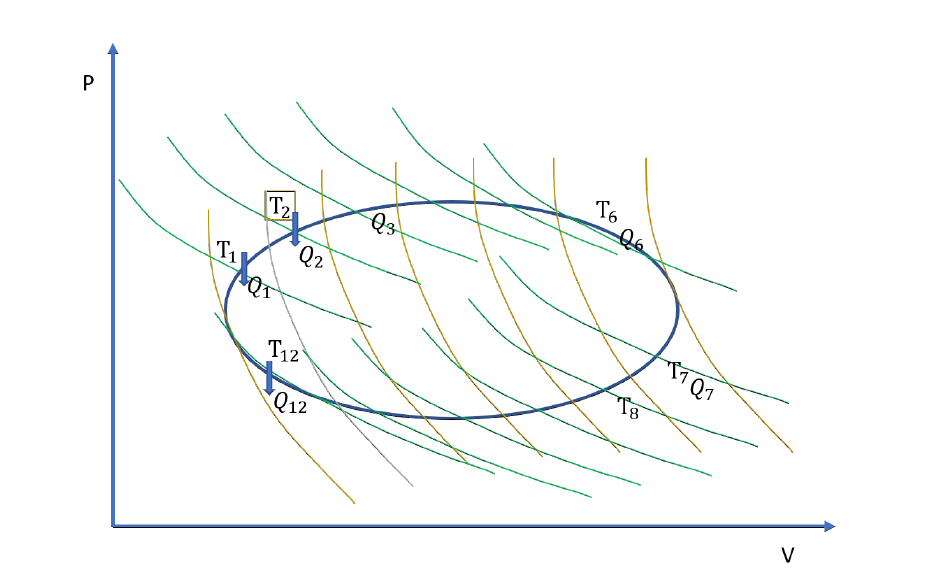
\includegraphics[scale=0.5]{teorema-clausius-3.png}
\caption{aproximación del ciclo por finitos ciclos de carnot}
\label{fig:5-2}
\end{figure}

Como cada ciclo de carnot cumple que:

$$ \dfrac{Q_1}{Q_2} = \dfrac{T_1}{T_2} \Longrightarrow \dfrac{Q_1}{T_1} = \dfrac{Q_2}{T_2} \Longrightarrow \dfrac{Q_1}{T_1} - \dfrac{Q_2}{T_2} = 0 $$

Entonces el cualquier ciclo (hemos supuesto un ciclo genérico cualquiera) cumplirá que:

\begin{equation}
 \sum_i^n \dfrac{Q_i^{\pm}}{T_i}=0  
\end{equation}

Como podemos suponer que hay infinitos ciclos de carnot (infinitamente cerca unos de otros) tenemos que:

\begin{equation}
\oint \dfrac{\D ' Q}{T} = 0
\end{equation}

\Teorema{\textbf{Teorema de clausius:} el teorema de clausius nos dice que para cualquier ciclo (ya que todo ciclo admite su substitución por ciclos de carnot y la integral es 0 si es reversible) cumple que:
$$ \oint \dfrac{\D ' Q}{T} = 0 $$ 
siendo $\D ' Q$ el calor que absorbe el sistema en cada proceso infenitesimal y $T$ la temperatura de la fuente exterior al sistema.} \\ \\

Aunque veamos que $\D ' Q$ no es una diferencial exacta $\D ' Q / T$ si (deja el estado en la misma situación). A esta nueva diferencial exacta le llamaremos \textbf{entropía (S)} y será:

\begin{equation} 
\D S = \parentesis{\dfrac{\D ' Q}{T}}_{rev}   
\end{equation}

Y por lo tanto necesariamente para un proceso reversible debe cumplirse que:

\begin{equation}
S_B - S_A = \int_A^B \left( \dfrac{\D ' Q}{T} \right) _{rev}
\end{equation}
Recordemos que todos los procesos adiabáticos $\D Q=0$. TOdos los procesos adabáticos y reversibles $\D S = 0$, que se llamaran procesos \textbf{isoentrópicos}. Si un proceso es isoentrópico la entropía se mantiene constante. \\

Además podemos reescribir el primer y segundo principios como:

\begin{equation}
\D U = T \D S + P \D X
\end{equation}

De esto se puede deducir que la entropía es una variable termodinámica extensiva aditiva, ya que dependerá del tamaño del sistema. En este caso U, X, P, T y S son variables de estado y dicho enunciado una relación entre ellas en la que no influyen los procesos (dependen solo del estado del sistema y no del recorrido o proceso por el que llegan a dicho estado).  \\


Sin embargo existen ciertas objeciones para todo lo dicho anteriormente:

\begin{enumerate}
\item El argumento depende de la hipótesis, ya que el sistema no tendría porque existir en todos los estados que interviene en la subdivisión (y por lo  tanto que no se pudiera aproximar por ciclos de carnot).

\item No se ha demostrado el resultado para superficies adiabáticas de más de dos variables (dos coordenadas extensivas, por ejemplo). \\
\end{enumerate}

\subsection{Segundo principio de la termodinámico: principio de aumento de entropía}

En este punto trataremos los aspectos no reversibles del Segundo Principio que nos conducirán al principio de aumento de la termodinámica. Los aspectos no reversibles del segundo principio se obtienen de la parte no reversible del ciclo de Carnot que establece que de todas las máquinas que funcionan entre dos focos dados la que funciona de manera reversible es la que tiene mas rendimiento:

$$ \eta_c \geq \eta \Longrightarrow 1 - \dfrac{Q_{1c}}{Q_{2c}} \geq 1 - \dfrac{Q_1}{Q_2} \Longrightarrow \dfrac{Q_{1c}}{Q_{2c}} \leq \dfrac{Q_1}{Q_2} $$

Y esto implica directamente que:

$$  \dfrac{Q_{1c}}{Q_{2c}} = \dfrac{T_1}{T_2} \leq \dfrac{Q_1}{Q_2}  \Longrightarrow \dfrac{Q_2^+}{T_2} + \dfrac{Q_1^-}{T_1} \leq 0 $$ \\

Se verifica la igualdad cuando el proceso es reversible y la desigualdad cuando es irreversible. En general se obtiene que para un ciclo general que no son reversibles obtenemos \textbf{la relación de Clausius} que nos dice que:

\begin{equation}
\oint \dfrac{\D ' Q}{T} \leq 0 \label{Ec:5-relacion-clausius}
\end{equation}

Hay que tener cuidado cuando ahora hablamos de $\D ' Q$, antes interpretado como el calor transferido entre dos estados infinitamente próximos pero que ahora, como estamos en procesos no reversibles no se tiene porque dar la sucesión de estados de equilibrio. Consideremos ahora el siguiente sistema:

\begin{figure}[h!] \centering
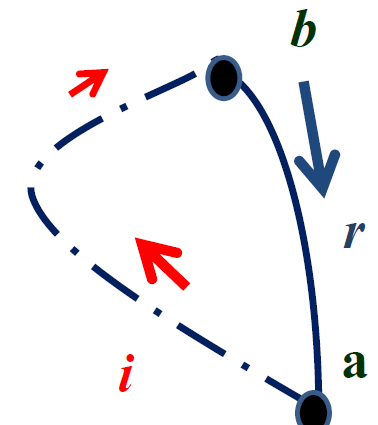
\includegraphics[scale=0.7]{Desigualdad-clausius.png}
\end{figure}

Consideremos el proceso i irreversible y el proceso r reversible. Como este proceso no es reversible se cumplirá \ref{Ec:5-relacion-clausius} y como hay un proceso reversible pero otro no tenemos que: \\

$$ \oint \dfrac{\D ' Q}{T} = \int_a^b  \dfrac{\D' Q}{T} + \int_b^a  \dfrac{\D' Q}{T} = \int_a^b  \dfrac{\D' Q}{T}  + S_a - S_b \leq 0 $$ \\

Y directamente de esto se deduce la \textbf{desigualdad de clausius}:

\begin{equation}
\int_a^b  \dfrac{\D' Q}{T}  \leq S_b - S_a
\end{equation}

De la desigualdad de clausius podemos tener que para 3 procesos la variación de entropía será: 
\begin{itemize}
\item \textbf{Proceso irreversible:} en este caso el calor intercambiado no es cero y por ser irreversible se cumple la desigualdad: $$ \int_a^b  \dfrac{\D' Q}{T} + S_a < S_b $$ \\
\item \textbf{Proceso irreversible adiabático:} por ser adiabático el calor intercambiado es cero pero por ser irreversible se cumple la desigualdad $$ S_a < S_b  $$\\
\item \textbf{Proceso reversible (y adiabático):} por ser reversible es adiabático, y por ello el calor intercambiado es 0 y se cumple la igualdad: $$ S_a = S_b $$\\
\end{itemize}

Entonces por esto en cualquier sistema aislado, que no permita intercambio de energía interna del sistema (ya que de ser así probablemente se modifique también la entropía, ya que es función de estado) se cumplirá que la entropía   total del sistema siempre que se realice un proceso dentro de él sistema aumentará, o en su defecto (únicamente para procesos reversibles) permanecerá constante. \\


Como el universo es un sistema aislado la cualquier evolución que ocurra en ella (por necesidad) tiene que implicar un aumento de entropía. Eso nos da un sentido de evolución de los procesos termodinámicos, que era una de las motivaciones por las que desarrollamos toda esta teoría: conocer el sentido de los procesos. \\

Entonces tenemos todos los conocimientos necesarios para enunciar el segundo principio de la termodinámica, que nos dice que: \\

\Teorema{\textbf{\underline{Segundo principio de la termodinamica:}} la entropía no destruirse pero puede crearse, ya que la entropía de un sistema aislado crece siempre o en el ímite permanece constante (en el caso de proceso reversible): $$ (S_b - S_a)_{aisld} = (\Delta S)_{aisld} \geq 0 \Longleftrightarrow S_b \geq S_a $$} \\ \\

Mientras que la primera ley nos decía que la ``energía no puede crearse ni destruirse'' la segunda ley nos dice que la ``entropía puede crearse pero no destruirse''. \\

La \textbf{condición de entropía máxima} es \textbf{suficiente pero no necesaria} para demostrar que el sistema está en \textbf{equilibrio termodinámico} (en un sistema aislado). Es suficiente porque de encontrarse en entropía máxima el segundo principio imposibilita la realización de un proceso que disminuya la entropía y que sea máxima imposibilita que crezca. No es necesaria porque el segundo principio no imposibilita en ningún momento . \\

\subsection{Trabajo máximo y degradación de la energía}
Consideremos un sistema que sufre una evolución entre dos estados infinitamente próximos. Según la expresión general del primer principio se cumple 	que:

$$\D U = \D ' Q + \D ' W$$

Ahora vamos a estudiar como el segunda principio impone una restricción acerca del trabajo máximo que puede obtenerse del sistema. En general el primer principio puede enunciarse de dos maneras diferentes en función de si sufre un proceso reversible o si sufre un proceso irreversible: \\


\begin{equation}
\left\lbrace \begin{array}{l l}
\D U = T \D S + \D ' W_r & \text{reversible}\\ 
\D U = \D ' Q + \D ' W_i & \text{irreversible}\\ 
\end{array} \right.
\end{equation} \\


Suponemos que del estado a al estado b vamos por dos caminos. Uno de ellos es un proceso reversible y otro un proceso reversible. Como la energía interna solo depende de a y b, la diferencia en ambos procesos debe ser la misma. Además sabemos por el segundo principio de la termodinámica:  

$$ \D'  Q_i < T \D S $$ 

Entonces por el simple hecho de que la variación de energía interna debe ser la misma tenemos que los trabajos ejercidos por el medio deben compensar esto . Entonces si escribimos los trabajos como:


\begin{equation}
\left\lbrace \begin{array}{l l}
\D ' W_r = \D U - T \D S & \text{reversible}\\ 
\D ' W_i = \D U - \D ' Q  & \text{irreversible}\\ 
\end{array} \right\rbrace \Longrightarrow \D ' W_r < \D ' W_i
\end{equation} \\


Ahora tendríamos que estudiar el criterio de signos de todo esto, pero antes de ello vamos a estudiar un poco, y de manera cualitativa, las implicaciones que tiene esto en el sistema. Realmente cuando hablamos de que el trabajo realizado de forma reversible por el medio es menor que el irreversible lo que queremos decir es que, para hacer el mismo proceso, para cambiar la misma cantidad de energía interna de un proceso necesitamos el medio necesita realizar mucho mas trabajo, por lo que es menos eficiente. En este caso hablamos de trabajo ejercido por el medio, y por eso el criterio de signos es positivo. Ahora bien, podemos hablar de trabajo ejercido por el sistema, en cuyo caso debemos cambiar el signo del trabajo y:

$$ \D ' W_r^- > \D ' W_i^- \Longrightarrow |\D ' W_i^- | >  |\D ' W_r^- | $$

Entonces como podemos ver si el proceso conlleva una irreversibilidad el trabajo realizado por el sistema (negativo) es menor (mas negativo) que el realizado de manera reversible, y por lo tanto, menos eficiente. El trabajo que realiza el sistema a mayores se convierte en calor disipativo que se transfiere al sistema, y no se usa en realizar el cambio de energía interna. Por eso mismo un proceso irreversible es menos eficiente que un proceso reversible.  \\

Si ahora estudiamos el intercambio de calor entre el sistema y el medio podremos darnos cuenta de que el calor recibido por el medio (desde el sistema) es mucho mayor si trasferimos el calor con un proceso reversible que con un proceso irreversible:

$$ T \D S  = D ' Q_r^+ > \D'  Q_i $$

Y el calor que trasmite el sistema al medio es mayor si se trasmite de forma reversible que de forma reversible, ya que:

$$ -T \D S = D ' Q_r^- < \D ' Q_i $$
 

Ahora  vamos a estudiar el concepto de la degradación de energía. Para  poder definirlo primero supondremos algunas hipótesis. Supongamos un esquema como el de la figura siguiente, donde hay 3 focos calientes, extrayendo del foco mas caliente un calor $Q_2^+$, que será la misma cantidad de calor que se extraerá del calor del foco caliente $t_3$. La única diferencia "apreciable" será la temperatura del foco del que el ciclo que estudiamos, que en un caso es menor:

\begin{figure}[h!] \centering
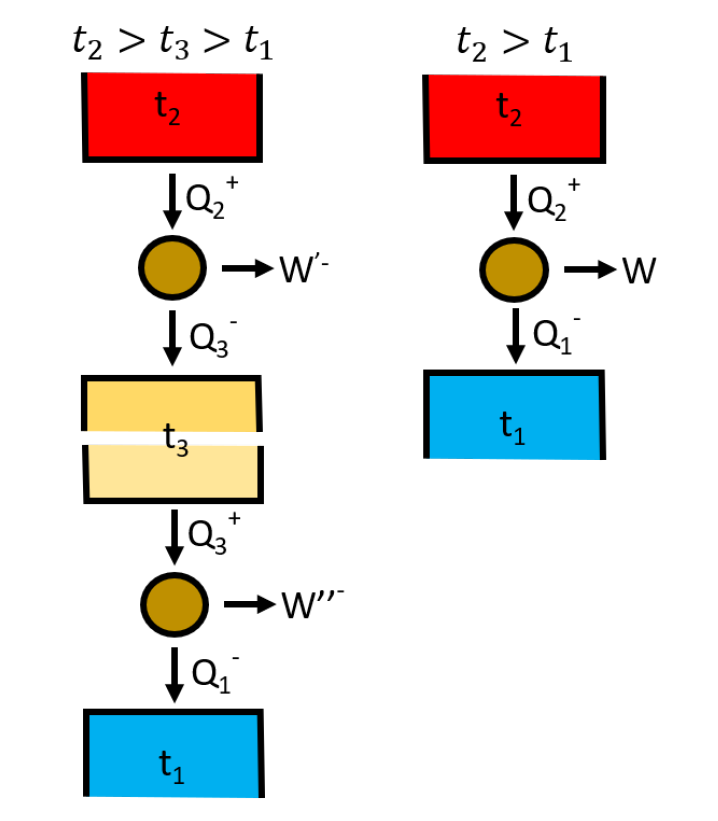
\includegraphics[scale=0.6]{Temperatura-absoluta-carnot.png}
\caption{2 máquinas donde $Q_3^+ = Q_2^+$. No son máquinas equiavalentes.}
\label{fig:5-degradacion-energia}
\end{figure}

Sabemos que el trabajo máximo se extrae de los procesos reversibles, y por ser reversibles podemos aproximarlos por finitos o procesos de carnot, y como en los ciclos de carnot el rendimiento de la máquina solo depende de la temperatura de los focos tenemos que:

$$ W_{max}' - W_{max}'' = Q_2^+ \left( 1 - \dfrac{T_1}{T_2} \right) - Q_2^+ \left( 1 - \dfrac{T_1}{T_3} \right) = Q_2 T_1 \left( \dfrac{T_2-T_3}{T_3 T_2} \right) > 0 \Longrightarrow $$

$$ W_{max}' - W_{max} '' > 0 \Longrightarrow W_{max}' > W_{max}'' $$

Es decir cuanto menor sea la temperatura de un sistema, menor es su capacidad de producir trabajo tomando la misma cantidad de calor. En este sentido se habla de \textbf{degradación de energía}. Cuando una cierta cantidad de calor pasa de un sistema otro de temperatura mas baja la energía es la misma pero su capacidad de producir trabajo es menor. 


\subsection{Aplicaciones técnicas del principio de aumento de entropía}

Los procesos reales son irreversibles, entonces para ellos se puede aplicar el principio de aumento de entropía. Vamos a ver qué trabajo máximo o rendimiento máximo podemos conseguir en motores térmicos y frigoríficos. \\

\subsubsection{Trabajo limite para la máquina térmica}
El \textbf{trabajo límite} que no puede superar una máquina térmica corresponde a: \\

$$ W^+ = Q_2^+ \left[  \parentesis{1- \frac{T_1}{T_2}} \right] $$ \\


Es decir en los procesos reales el trabajo que se puede conseguir con una máquina térmica debe cumplir siempre que: \\

\begin{equation} 
W^+ < Q_2^+ \left[ \parentesis{- \frac{T_1}{T_2}} \right] 
\end{equation} \\

Vamos a intentar demostrarlo. Como una máquina térmica funciona por ciclos:

$$ \Delta U = Q_2^+ - Q_1^- + W^- = 0 \Longrightarrow   Q_1^+ = Q_2^+ + W^-$$ \\

Y como es un proceso que ocurre en el universo tenemos que: \\

$$ \Delta S  = \Delta S_{maq}+ \Delta S_{foco frio} + \Delta S_{foco caliente} \leq 0; \ \Delta S_{maq} = 0 \ \ (\text{ciclo}) $$ \\

De lo que se puede extraer que (recordemos que los signos del calor vienen de que valoramos el calor que sale o entra respecto cada foco frío/caliente): \\

$$ \Delta S = \Delta S_{ff} + \Delta S_{fc} = \dfrac{Q_1^+}{T_1} + \dfrac{Q_2^-}{T_2} = \dfrac{Q_2^+ + W^-}{T_1} - \dfrac{Q_2^+}{T_2} \geq 0  \Longrightarrow $$

$$ \dfrac{W^-}{T_1} \geq Q_2 \parentesis{\dfrac{1}{T_2}-\dfrac{1}{T_1}} = Q_2 \parentesis{\dfrac{1}{T_2}-\dfrac{1}{T_1}} \Longrightarrow $$  \\

$$  W^+ \leq  Q_2 \parentesis{1-\dfrac{T_1}{T_2}}$$ \\

Entonces siempre que el trabajo que podemos extraer de un foco caliente a través de un proceso cíclico no puede superar al mostrado, ese es en límite en la naturaleza. \\

\subsubsection{Trabajo límite para un frigorífico}

Si se trata de un frigorífico necesitamos un \textbf{trabajo mínimo requerido} para enfriar el foco frío: \\

\begin{equation}
W^+ > Q_1^+ \left[ \parentesis{\frac{T_2}{T_1}-1} \right]
\end{equation}  \\

Que se puede demostrar de manera similar que la máquina térmica, usando la entropía, siendo $T_1$ la temperatura del foco frío, $T_2$ la del foco caliente, $Q_1$ el calor que sacamos del foco frío y $Q_2$ el que enviamos al foco caliente (esta vez haremos los cálculos del tirón): \\

$$ \Delta U = Q_2^- + Q_1^+ + W^+ = 0 \Longrightarrow Q_2^+ = Q_1^+ + W^+ $$ \\
$$ \Delta S = \Delta S_{maq} + \Delta S_{ff} + \Delta S_{fc}; \ \Delta S_{maq } = 0 \ (\text{por ser ciclo}) \Longrightarrow $$ \\
$$ \Delta S_{ff} + \Delta S_{fc} = \dfrac{Q_1^-}{T_1} + \dfrac{Q_2^+}{T_2} \geq 0 \Longrightarrow  \dfrac{Q_1^-}{T_1} + \dfrac{Q_1^+ + W^+}{T_2} \Longrightarrow \dfrac{W^+}{T_2} \geq Q_1^+ \parentesis{\dfrac{1}{T_1}-\dfrac{1}{T_2}} \Longrightarrow $$ \\
$$  W^+ \geq Q_1^+ \left[ \parentesis{\dfrac{T_2}{T_1} - 1} \right] $$ \\

\subsubsection{Trabajo límite para una nevera}

Podemos estudiar el caso de un frigorífico real donde el sistema que se enfría no es un foco frío si no el interior de un sistema aislado adiabáticamente que llamaremos \textbf{nevera}. Entonces el trabajo mínimo necesario para enfriar una nevera será:

\begin{equation}
 W^+ \geq -T_2 \Delta S_{nev} - Q_1^+ 
\end{equation}

cumpliéndose la igualdad para aquellos procesos no reversibles. Podemos imaginarnos una nevera como un sistema aislado adiabáticamente con una capacidad calorífica $C_x$ tal que:

$$ C_x \D T = \D Q \ (\text{a x constante}) $$

Entonces podemos deducir que:

$$ \Delta S_{nev} + \Delta S_{fc}  = \Delta S_{nev} + \dfrac{(Q_1^+ + W^+)}{T_2} \geq 0  \Longrightarrow \dfrac{W^+}{T_2} \geq \Delta S_{nev} - \dfrac{Q_1^+}{T_2} $$

Por lo que queda demostrada dicha relación.

\newpage

\section{Sistemas abiertos}
\subsection{Formulación general de las variables termodinámicas}

La combinación del Primer y Segundo Principio nos había dado para un sistema cerrado:

\begin{equation}
\D U = T \D S + \sum_i P \D X_i
\end{equation}

Para un sistema simple la coordenada extensiva es única (solo hay uno). Hasta que se diga lo contrario supondremos que estudiamos un sistema simple, aunque podremos generalizarlo para mas coordenadas intensivas con facilidad. \\

Las 5 variables $U$, $S$, $T$, $P$ y $X$ son variables de estado, no dependen del proceso, y dicha ecuación acaba siendo una relación de la  termodinámica que no depende del proceso (del camino). Esta relación está marcando nos está mostrando que la energía interna $U$ es una variable de estado que depende de $S$ y de $X$, de tal forma que:

\begin{equation}
U = U(S, X)
\end{equation}

Y de lo anterior se puede deducir fácilmente que:

\begin{equation}
\parentesis{\parciales{U}{S}}_X = T; \ \parentesis{\parciales{U}{X}}_S = P
\end{equation}

Una vez visto esto podemos entender una cosa: todas las variables se relacionan entre sí, de lo que podemos deducir que de las 5 coordenadas termodinámicas podemos extraer en total 10 funciones, algunas con mas relevancia que otras. Algunas ya las hemos visto, solo que ahora las escribiremos con nombres y apellidos:

\begin{itemize}
\item \textbf{Ecuación fundamental:} juega un papel muy importante ya que de esta se derivan todas las demás ecuaciones, mediante derivaciones y substituciones. Esta ecuación es:

\begin{equation}
U = U(S,X)
\end{equation}

Su forma diferencial, llamada \textbf{ecuación de Gibbs} o \textbf{ecuación diferencial fundamental} viene dada por:

\begin{equation}
\D U = T \D S + P \D X
\end{equation}

La ecuación fundamental proporciona una información completa del estado termodinámico de un sistema.

\item \textbf{Ecuaciones de estado:} se obtienen de derivar la ecuación fundamental dejando una de las coordenadas extensivas constantes y despejar la coordenada intensiva restante, y como $U$ se puede reescribir en función de $S$ y $X$:

\begin{equation}
T = \parentesis{\parciales{U}{S}}_X = T(S,X) ; \ P = \parentesis{\parciales{U}{X}}_S = P(S,X)
\end{equation}

\item \textbf{Ecuación térmica de estado:}  podemos obtener las variables $U$, $S$ y $X$ en función de las coordenadas intensivas reescribiendo y derivado la ecuación fundamental. La ecuación térmica consiste en reescribir la variable $X$ en función de las coordenadas intensivas:

\begin{equation}
X = X(T, P)
\end{equation}

O también pueden relacionar las ecuaciones intensivas con el resto: 

\begin{equation}
P = P(T, X)
\end{equation}

\item \textbf{Ecuación calórica de estado:} si despejamos la energía interna $U$ en función de la temperatura y la coordenada extensiva podremos obtener la ecuación calórica de estado:

\begin{equation}
U = U(T,X)
\end{equation}

\end{itemize}

Todo esto se ha realizado en el lenguaje energía, pero podría reenunciarse para el lenguaje entropía. Cuando hablamos de lenguaje entropía o lenguaje energía en realidad nos estamos refiriendo a cual es la variable que despejamos en la ecuación fundamental. Tal y como lo hemos hecho antes hemos despejado la energía interna, pero sabemos que podemos despejarla en función de la entropía de tal forma que obtendríamos la \textbf{ecuación fundamental en forma entropía:}

\begin{equation}
S = S(U, X)
\end{equation}

Y su forma diferencial:

\begin{equation}
\D S = \dfrac{1}{T} \D U + \dfrac{P}{T} \D X \label{Ec:6-diferencial-entropia}
\end{equation}

Y como antes:

\begin{equation}
\dfrac{1}{T} = \parentesis{\parciales{S}{U}}_X; \ \dfrac{P}{T} = \parentesis{\parciales{S}{X}}_U
\end{equation}

Ahora cambiando T por S:

\begin{equation}
\D S = \parentesis{\parciales{S}{T}}_X \D T + \parentesis{\parciales{S}{X}}_T \D X
\end{equation}

De lo que podemos extraer las capacidades caloríficas a P y X constantes. Si imponemos en la ecuación \ref{Ec:6-diferencial-entropia} la siguiente restricción $X = \text{cte}$ tenemos que:

$$ \D S  =  \parentesis{\parciales{S}{T}}_X \D T \Longrightarrow \ \D' Q_X = T \D S =  T \parentesis{\parciales{S}{T}}_X \D T \Longrightarrow  C_X = T \parentesis{\parciales{S}{T}}_X $$

Y lo mismo para $P =$cte:

$$ C_P = T \parentesis{\parciales{S}{T}}_P $$

\subsection{Generalización del segundo principio para sistemas abiertos}

Hasta ahora habíamos impuesto dos restricciones a nuestro sistema: tenía que ser simple y cerrado (no puede intercambiar materia). Ahora vamos a tratar de generalizar todas estás ecuaciones y relaciones para sistemas abiertos (pueden intercambiar materia). En realidad generalizar todos lo visto hasta ahora para sistemas abiertos no es para nada trivial, ya que conceptos como trabajo o calor dejan de encontrar sentido. \\

El problema se reduce a que no somos capaces de encontrar coordenadas de deformación adecuadas para las variaciones de masa, ya que hasta ahora hemos omitido usar como variable de estado las masas de los componentes de un sistema. Esto se hace porque la masa no es ajustable adiabáticamente. Para solucionar este conflicto podemos optar por dos caminos: 

\begin{enumerate}
\item Reconstruír toda la termodinámica de tal forma que desde el principio incluya la masa como variable de estado.

\item Generalizar los resultados obtenidos hasta ahora y examinar todas las posibles consecuencias experimentales, que luego experimentalmente se verificará, obteniendo así un fundamento empírico de la generalización. 
\end{enumerate}


Lo primero que debemos hacer es buscar nuevas coordenadas parar explicar la nueva situación de intercambios másicos (sistemas físico-químicos). Entonces en nuestro nuevo sistema que constará de F \textbf{fases} (una fase es un estado de un sistema homogéneo (sistema que es aquel que tiene todas las coordenadas termodinámicas iguales en todos los puntos del espacio)) cada una constituida por c sustancias químicas distintas (componentes). Una fase puede ser el estado de cierto componente, como líquido, gaseoso... \\

Para describir el equilibrio termodinámico de este tipo de sistemas  tendremos las típicas y conocidas variables extensivas $X_i$ y unas nuevas que indiquen la composición del sistema, que denominaremos coordenadas químicas. La composición de un sistema fisico-químico puede variar por:

\begin{itemize}
\item Intercambios de componentes a través de la membrana del sistema.
\item Trasformación de componentes mediante reacciones químicas en el seno de las fases.
\item Paso de componentes a través de la superficie de separación entre fases. Por ejemplo si en una pota tenemos agua en estado líquido o en estado gaseoso, y tenemos que esta en ebullición, la componente de cada fase del agua está variando. Se considera componente a un elemento y su estado.
\end{itemize}

Supongamos unas hipotesis parar empezar a desarrollar todo el aparato matemático. En primer lugar supondremos que nuestro sistema es \textit{homogéneo} y \textit{químicamente inerte}, con una fase en la que no tienen lugar reacciones químicas, y en consecuencia las coordenadas químicas no tienen dependencia entre sí, siendo la coordenada química elegidas el número de moles de cada  substancia $n_i$. La única forma de variar la composición del sistema es a través de su frontera. Ahora si la temperatura y las coordenadas extensivas se mantienen constantes, y se introduce una infenitesimal cantidad del compuesto j $\D n_j$ (a la misma temperatura que el sistema), tenemos que será necesario aportar un trabajo proporcional a la cantidad de composición transferida. A la constante que relaciona trabajo y cantidad de composición intercambiada se el llama \textbf{potencial químico} $\mu_j$. Entonces para cualquier proceso tenemos que:

\begin{equation}
\D ' W = \sum_{i=0}^n P_i \D X_i + \sum_{j=0}^m \mu_j \D n_j
\end{equation}

Y por lo tanto podemos reescribir la \textbf{ecuación diferencial de Gibbs} en lenguaje energía y entropía como:

\begin{equation}
\D U  = T \D S + \sum_{i=0}^n P_i \D X_i + \sum_{j=0}^m \mu_j \D n_j 
\end{equation}


\begin{equation}
\D S  =  \dfrac{1}{T} \D U + \sum_{i=0}^n \dfrac{P_i}{T} \D X_i + \sum_{j=0}^m \dfrac{\mu_j}{T} \D n_j  
\end{equation}

De lo que podemos extraer las mismas conclusiones (existencia de energía interna, entropía, temperatura) que hasta ahora solo que incluyendo las coordenadas químicas. 

\subsection{Ecuación fundamental del sistema pluricomponente}
Al igual que antes, podemos escribir tanto la ecuación fundamental como las ecuaciones térmicas, calóricas... en función de las componentes anteriores (T,P,V, S o U) y las nuevas componentes másicas (n, $\mu$). Entonces las ecuaciones mas relevantes desde el punto de vista de información termodinámica con todas las variables:

\begin{itemize}

\item \textbf{Ecuación fundamental:} las ecuaciones fundamentales ahora dependerán de todas las variables. Recordemos qu estas ecuaciones deben ser, por definición, homogéneas de primer grado respecto las variables:

\begin{gather}
\begin{array}{ll}
U & = U(S, X_1,\ldots,X_n,n_1,\ldots,n_c) \\
S & = S(U, X_1,\ldots,X_n,n_1,\ldots,n_c)
\end{array}
\end{gather} \\

\begin{gather}
\begin{array}{ll}
\lambda U(S, X_1,\ldots,X_n,n_1,\ldots,n_c) & = U(\lambda S, \lambda  X_1,\ldots, \lambda X_n, \lambda n_1,\ldots, \lambda n_c) \\
\lambda S(U, X_1,\ldots,X_n,n_1,\ldots,n_c) & = S(\lambda U, \lambda X_1,\ldots,\lambda X_n, \lambda n_1,\ldots,\lambda n_c)
\end{array}
\end{gather}


\item \textbf{Forma de Euler}: eas ecuación fundamental por ser homogénea de primer grado puede escribirse con la \textit{forma de Euler} (revisar \ref{sub:anex-homogenea}):

\begin{equation}
U = \parentesis{\parciales{U}{S}}_{X_i, n_i} S + \sum_{i=1}^s \parentesis{\parciales{U}{X_i}}_{S, X_{j\neq i}, n_i} X_i + \sum_{i=1}^s \parentesis{\parciales{U}{n_i}}_{S, n_{j\neq i}, X_i} n_i 
\end{equation}

\begin{equation}
S = \parentesis{\parciales{S}{U}}_{X_i, n_i} U + \sum_{i=1}^s \parentesis{\parciales{S}{X_i}}_{U, X_{j\neq i}, n_i} X_i + \sum_{i=1}^s \parentesis{\parciales{S}{n_i}}_{U, n_{j\neq i}, X_i} n_i 
\end{equation} \\

Que lleva directamente a la \textit{relación de euler} ya que como hemos visto antes las coordenadas intensivas conjugadas de cada extensiva $Y$ son las derivadas parciales entre energía y coordenada extensiva $Y$ con el resto de coordenadas extensivas constantes, entonces:

\begin{equation}
U = TS + \sum_{i=1}^s P_i X_i + \sum_{i=1}^r \mu_i n_i 
\end{equation}
\begin{equation}
S = \frac{1}{T} U  +  \sum_{i=1}^s \frac{P_i}{T} X_i  + \sum_{i=1}^r \frac{\mu_i}{T} n_i 
\end{equation}

Cualquier parámetro intensivo se puede obtener como función de las coordenadas extensivas,  químicas y la energía interna o entropía (obteniendo la representación energía interna o la representación entropía). Tener todas las coordenadas intensivas desde un punto de vista de información termodinámica es el misma que tener la ecuación fundamental.

\item \textbf{Ecuaciones de estado:} se denominan como ecuaciones de estado a las ecuaciones que relacionan cada una de las coordenadas intensivas con las extensivas, tanto en representación energía como entropía. La característica principal de las ecuaciones de estado es que son homogéneas de grado cero. Es una implicación directa de que la ecuación fundamental sea homogénea de primer grado:

\begin{gather}
\begin{array}{lll}
T(S, X_1, \ldots, X_s, n_1, \ldots, n_r) & = & T(\lambda S, \lambda X_1, \ldots, \lambda X_s,\lambda n_1, \ldots, \lambda n_r)  \\
P_i(S, X_1, \ldots, X_s, n_1, \ldots, n_r) & = & P_i(\lambda S, \lambda X_1, \ldots, \lambda X_s,\lambda n_1, \ldots, \lambda n_r) \\
\mu_i (S, X_1, \ldots, X_s, n_1, \ldots, n_r) & = & \mu_i (\lambda S, \lambda X_1, \ldots, \lambda X_s,\lambda n_1, \ldots, \lambda n_r)
\end{array}
\end{gather}


Además estas ecuaciones no son todas independientes entre sí, debido al carácter homogéneo de primer grado de la ecuación fundamental. Una relación (diferencial, pero relación al fin y al cabo) la podemos hallar al diferencial la ecuación de euler, de donde podemos obtener que la \textbf{relación de Gibbs-Duhem}:

\begin{equation}
S \D T + \sum X_i \D P_i + \sum n_i \D \mu_i = 0
\end{equation}

El conocimiento de todas menos una de las ecuaciones de estado es equivalente a conocer la ecuación fundamental mas una constante de integración indeterminada.

\item  \textbf{Ecuación calorífica:} la ecuación calorífica es la expresión de la energía interna en función de las coordenadas extensivas y la temperatura. Conocer la ecuación calorífica no equivale a conocer la ecuación fundamental. 


\begin{equation}
U = U(T, X_i, n_i)
\end{equation}

\item \textbf{Ecuaciones térmicas de estado:} las ecuaciones térmicas de estado permiten escribir las coordenadas intensivas en función de la temperatura y las coordenadas extensivas:

\begin{equation}
P_j = P_j (T, X_i, n_i)
\end{equation}

El conocimiento pleno de la ecuación calorífica y las ecuaciones térmicas equivale a conocer la ecuación fundamental.

\end{itemize}

%\begin{itemize}
%\item \textbf{Ecuación fundamental:} en este caso las ecuaciones fundamentales en relación entropía y energía son iguales que la anterior ecuación fundamental solo que tendríamos que añadir las coordenadas intensivas y extensivas químicas de tal manera que:
%\item \textbf{Ecuación fundamental diferencial:}
%\item \textbf{Relación de Gibbs-Duhmen:}
%\item \textbf{Ecuaciones de estado:}
%\item \textbf{Ecuación térmica de estado:}
%\item \textbf{Ecuación calórica de estado:}
%\end{itemize}

\newpage

\section{Potenciales termodinámicos}

Es bastante sencillo de intuir que son las algunas magnitudes como intensidad, volumen, presión, temperatura... sin embargo algunas otras como la energía interna o la entropía son un poco mas complicadas de entender, siendo, por lo general, bastante abstractas. Lo mismo es para calcularlas, es bastante sencilla calcular la presión de una habitación, sin embargo su entropía es directamente imposible (no existe un ``entropimetro'' ni nada parecido). Ahora bien, en las fórmulas termodinámicas vistas hasta ahora todos los procesos dependen, en mayor o menor medida, de estas coordenadas imposibles de calcular; y los sistemas están definidos por esto. Como podemos imaginar, este es un gran problema a la hora de intentar conocer toda la información termodinámica de un sistema. Por eso en este tema nos preguntamos, ¿Existe alguna manera de replantear el formalismo matemático visto hasta ahora de tal forma que substituíamos estas coordenadas en otras mas sencillas de calcular, como las intensivas temperatura o presión? A lo largo del tema comprobaremos si realmente esto es posible, y trataremos de describir completamente el estado de un sistema termodinámico con estas coordenadas. \\

\subsection{Trasformada de legendre}

Sea la función matemática $y = y(x_1,x_2,x_3 \ldots, x_n)$. Tenemos que conseguir que las diferenciales $p_i$ definidas como:

\begin{equation}
p_i = \parciales{y}{x_i}
\end{equation}

Sean las nuevas variables independientes, de una manera biyectiva, para que podamos recosntruír la variable de partida a partir de la nueva función, y de esta forma no perder ningún tipo de información termodinámica. \\

Planteemos el problema, de momento, con una función $y=y(x)$. La pendiente para cada valor de $x$ es:

\begin{equation}
p = \dfrac{\D y}{\D x } = y' (x)
\end{equation} 

Como $y'(x)$ es una función de $x$ y la igualamos a p podemos despejar $x$ obteniendo una función $x = x(p)$, y podemos redefinir la función $y$ como $y = y(x(p)) = g(p)$. Sin embargo si lo hacemos de esta forma perdemos información, ya que $y=g(p)$ es una ecuación diferencial cuya integral da una constante de integración indeterminada, ya que entonces si hacemos el cambio tendríamos $y = y(x) + \cte$, teniendo una familia de curvas en el plano $x-y$.  Entonces este cambio así no nos sirve. Quizás el problema es el punto de vista desde el que miramos la curva: ahora mismo estamos suponiendo que una curva es el lugar geométrico de los puntos que satisfacen la ecuación $y=y(x)$. Sin embargo también podemos verlo como la envolvente de una familia de tangentes a esa ecuación. Trataremos ahora el problema desde este nuevo punto de vista. \\

Ahora trataremos de establecer una trasformación entre el plano ($x, y(x)$) y $\Psi(p)$; tal que $p$ es la pendiente y $\Psi$ su coordenada en el origen para cada pendiente. La ecuación $\Psi$ nos da información sobre todas las tangentes a la curva en cada punto, asignando un valor de $\Psi$ a la pendiente $p$. Tenemos que:

\begin{equation}
y = \Psi + px 
\end{equation}  

Y despejando $p$ y $\Psi$ obtenemos que:

\begin{equation}
\Psi = y - px ; \ \ p = \dfrac{y - \Psi }{x}
\end{equation}

Y como antes podemos despejar $x$ en función de $p$, y como $y$ está en función de $x$, despejamos $y$ en función de $p$, podemos obtener la función $\Psi$ como una función de $p$ tal que $\Psi = \Psi(p)$. De esta forma obtendríamos una nueva ecuación termodinámica en función de las variables intensivas que contiene exactamente la misma información que la $y(x)$. Para comprobar que contiene la misma información termodinámica estudiaremos el proceso inverso: ¿Si tenemos la función $\Psi(p)$ podemos obtener la función $y(x)$? Veamos: \\

$$ \D \Psi = \D y - x \D p - p \D x = p \D x  -   x \D p - p \D x = - x \D p $$

Entonces tenemos que:

$$ - x = \dfrac{\D \Psi}{\D p} $$

Que como es una función de $p$ podemos despejarla y obtener $p = p(x)$ y por lo tanto despejando $y$:

$$ y = \Psi + px = \Psi(p(x)) + p(x) x = f(x) $$ 

Es decir: contienen la misma información termodinámica. Tras este planteamiento conocido como la \textbf{trasformada de Legendre} nos preguntamos por qué está forma de despejar $y$ con la coordenada en el origen funciona y por qué la otra no. Principalmente se debe a que cuando cogemos simplemente $p$ estamos escogiendo un grupo particular de curvas con esa pendientes en cada punto, pero en verdad hay multitud (infinitas) de curvas que compartan esa pendiente. Sin embargo si además definimos una coordenada en el origen para cada pendiente (es decir, definimos una recta) ya no existe una multitud de curvas, ya que si le sumamos una constante la coordenada cambiara esa constante. Por esa misma forma en este caso podemos hacer la inversa y volver a obtener $y(x)$.  \\

Todas estas consideraciones se pueden evaluar y generalizar para el caso de una función genérica  $y = y(x_1,x_2,x_3 \ldots, x_n)$, y podemos realizar la trasformación de Legendre solo para un grupo $k$ de variables independientes de tal forma que $\Psi = \Psi(p_1,p_2,p_3 \ldots,p_k, x_{k+1}, x_{k+2}, \ldots, x_n)$ obteniendo las siguientes relaciones importantes:

\begin{equation}
x_i = \parciales{\Psi}{p_i} \quad i \leq k 
\end{equation}

\begin{equation}
p_j = \parciales{\Psi}{x_j} \quad j > k
\end{equation}

\begin{equation}
\D \Psi = - \sum_{i=0}^k x_j \D p_i + \sum_{j=k+1}^n p_j \D x_j
\end{equation}

\begin{equation}
 y  = \Psi + \sum_{i=1}^k x_i p_i
\end{equation}

Una condición suficiente para la existencia de la trasformación es que el determinante del Jacobiando para $p_i$ y para $x_i$ sea distinto de 0. Es un problema similar al que hacemos en la mecánica clásica y el lagrangiano: muchas veces nos interesa mas obtener una función dependiente de algunos momentos generalizados en vez de velocidades generalizadas. Para esto realizamos una trasformación de Legendre obteniendo el Hamiltoniano. 

\subsection{Potenciales termodinámicos}
Como sabemos la ecuación fundamental contiene la máxima cantidad posible de información termodinámica en un sistema. La ecuación fundamental vista hasta ahora siempre se definió como energía interna o entropía en función de parámetros extensivos. Sin embargo esto acarrea dificultades experimentalmente, los intensivos serán aquellos que son mas fáciles de medir y controlar. Sean $X_i$ las coordenadas intensivas (incluyendo $S$ y $n$) y $P_i$ las intensivas, la trasformada de Legendre de la ecuación fundamental de $r$ coodenadas termodinámicas (mínimo 3, entropía, una por ser monocomponente y otra intensiva) de $k$ coordenadas intensivas:
 
 
\begin{equation}
\Psi_k = U - \sum_{i=1}^k P_i X_i
\end{equation}

A esta $\Psi_k$ se le llamará \textbf{potencial termodinámico}. En función de que coordenadas se trasformen obtendremos unos u otros potenciales, como el de Gibbs, Helmothz... \\

Ahora veremos las diferentes propiedades de los potenciales termodinámicos:

\begin{itemize}

\item  \textbf{Ecuación de Euler:} la ecuación de euler del potencial termodinámico viene dado por: 

\begin{equation}
\Psi_k = \sum_{j=k+1}^r X_j P_j
\end{equation}


Ya que $U = \sum_{i=1}^r X_i P_i$. 
\item \textbf{Ecuación de Gibbs o ecuación diferencial fundamental}. Como $\D U = \sum_{i=1}^r P_i \D X_i$ tenemos que:

\begin{equation}
\D \Psi_k =  - \sum_{i=1}^k X_i \D P_i + \sum_{j=k+1}^r P_j \D X_j 
\end{equation}

\item \textbf{Relaciones diferenciales:} tanto $X$ como $P$ están relacionadas diferencialmente de tal forma que:


\begin{equation}
\parciales{\Psi_k}{P_i} = X_i; \ \quad i = 1,2, \ldots, k
 \end{equation}

\begin{equation}
\parciales{\Psi_k}{X_i} = P_i; \ \quad i = k+1, k+2, \ldots, r
 \end{equation}

\item Las $\Psi_k$ son \textbf{ecuaciones homogéneas de primer grado} en los parámetros extensivos:

\begin{equation}
\Psi (P_1, P_2, \ldots, P_k, \lambda X_{k+1}, \ldots, X_{n}) = \lambda \Psi (P_1, P_2, \ldots, P_k, \lambda X_{k+1}, \ldots, X_{n})
\end{equation}

\item Al menos se necesita una coordenada extensiva para la descripción del sistema, consecuencia de que la ecuación fundamental sea homogénea de primer orden respecto a las variables extensivas. Si escribimos $\Psi_k(P_1, \ldots, P_k)$ tenemos que es una ecuación homogénea de grado 0, por lo que no contiene la misma información que la ecuación fundamental. Además si hacemos eso:

$$ \Psi_k = U - \sum_{i=1}^r P_i X_i =  \sum_{i=1}^r P_i X_i  -  \sum_{i=1}^r P_i X_i  = 0 $$


\item \textbf{Ecuación de Gibbs-Duhem:} si valoramos la ecuación de Gibbs del potencial $\Psi_r$ tenemos que:

\begin{equation}
\sum_{i=1}^r X_i \D P_i = 0
\end{equation}


\item \textbf{Ecuaciones de Gibbs-Helmholtz:} las ecuaciones de Gibbs-Helmholtz relacionan unos potenciales termodinámicos con otros. Por ejemplo sea el potencial $\Psi_k$ y $\Psi_j$ tal que $k>j$ podemos trasformar las $k-j$ variables restantes  de $\Psi_j$ para obtener $\Psi_k$ de tal forma que:


\begin{equation}
\Psi_k = \Psi_j - \sum_{i=j+1}^k P_i X_i; \quad \parentesis{\parciales{\Psi_k}{P_i}}_{j\neq i} = - X_i; \ \  \parentesis{\parciales{\Psi_k}{X_i}}_{j\neq i} = P_i
\end{equation}

Podemos reescribirlo: 

\begin{equation}
\Psi_k = \Psi_j + \sum_{i=j+1}^k P_i \parciales{\Psi_k}{P_i}
\end{equation}


\begin{equation}
\Psi_k = \Psi_j - \sum_{i=j+1}^k X_i \parciales{\Psi_k}{X_i}
\end{equation}

\item \textbf{Relaciones de Maxwell:} si la función matemática $f(x,y)$ es una función analítica cumple la condición:

$$ \dfrac{\partial^2 f}{\partial x \partial y} = \dfrac{\partial^2 f}{\partial y \partial x} $$

Como nuestros potenciales termodinámicos son diferenciales exactas lo cumplen y podemos reescribir la ecuación como:

\begin{equation}
\parciales{}{X_i} \parentesis{\parciales{f}{X_j}} = \parciales{}{X_j} \parentesis{\parciales{f}{X_i}} \Longrightarrow   \parciales{P_j}{X_i} = \parciales{P_i}{X_j}
\end{equation}

\begin{equation}
\parciales{}{P_i} \parentesis{\parciales{f}{X_j}} = \parciales{}{X_j} \parentesis{\parciales{f}{P_i}} \Longrightarrow   - \parciales{P_j}{P_i} = \parciales{X_i}{X_j}
\end{equation}

\end{itemize}

En un sistema mecánico conservativo la energía se puede almacenar en forma de energía potencial y posteriormente puede recuperarse. Bajo ciertas circunstancias esto es válido para sistemas termodinámicos. Se puede almacenar energía realizando trabajos sobre él. La energía que se almacena y posteriormente se recupera en forma de trabajo se llama energía libre. Existen muchas razones formas de energía libre, pero las cinco mas usadas son: la energía interna $U$, la entalpía $H$, energía libre de Helmholtz $F$, energía libre de Gibbs $G$ y el gran potencial $\Omega$. \\

\subsubsection{Ecuación fundamental en representación energía interna}

Sea un sistema fluido (se podría generalizar para cualquier sistema con una mínima coordenada intensiva) monocomponente, tenemos que la ecuación fundamental viene dado por:

\begin{equation}
U = U(S,V,n)
\end{equation}

Con las siguientes ecuaciones características:

\begin{itemize}
\item \textbf{Ecuación de Euler:} la ecuación de Euler es la representación de la energía interna en función de la entropía y las extensivas:

\begin{equation}
U = T S - p V+ \mu n
\end{equation}

\item \textbf{Ecuación de Gibbs:} es la ecuación de euler escrita en forma diferencial:

\begin{equation}
\D U = T \D S - p \D V + \mu \D n
\end{equation}

\item \textbf{Ecuación de Gibbs-Duhem:} si diferenciamos completamente la ecuación diferencial la ecuación de euler

\begin{equation}
S \D T - V \D p + n \D \mu = 0
\end{equation}

\item \textbf{Relaciones de Maxwell:} si reescribimos las relaciones de Maxwell para este sistema tenemos que:

\begin{equation}
\parentesis{\parciales{(-p)}{S}}_{V,n}  = \parentesis{\parciales{T}{V}}_{S,n} \quad \parentesis{\parciales{\mu}{S}}_{V,n} = \parentesis{\parciales{T}{n}}_{S,V} \quad \parentesis{\parciales{\mu}{V}}_{n,S} = \parentesis{\parciales{(-p)}{(n)}}_{V,S}
\end{equation}


\end{itemize}

\subsubsection{Entalpía}

La \textbf{entalpía} $H$ se obtiene al realizar la trasformada de Legendre de $U$ intercambiando el volumen por la presión, de tal forma que:

\begin{equation}
H = H(S,p,n)
\end{equation}

Tal y como vimos para un caso genérico, la trasformada de legendré será:

\begin{equation}
H = U - (-p)V = U + pV
\end{equation}

Entonces las ecuaciones características vendrán dadas por:

\begin{itemize}
\item \textbf{Ecuación de euler:} si cambiamos $U$ por $-Pv + TS + \mu n$ obtenemos que:

\begin{equation}
H = TS + \mu n
\end{equation}

\item \textbf{Ecuación de Gibbs:} si diferenciamos el potencial, como $\D U = T \D S -p \D V + \mu \D n$ tenemos que:

\begin{equation}
H = T \D S + V \D p + \mu \D n ; \quad \quad V = \parentesis{\parciales{H}{p}}_{S,n}
\end{equation}

\item \textbf{Relaciones de Maxwell:} en este caso tenemos que tener en cuenta que hay una intensiva en vez de una extensiva. Entonces podemos obtener:

\begin{equation}
\parentesis{\parciales{\mu}{S}}_{p, n} = \parentesis{\parciales{T}{n}}_{S,p} \quad \parentesis{\parciales{V}{S}}_{p, n} =  - \parentesis{\parciales{T}{(-p)}}_{S,n} \quad \parentesis{\parciales{V}{n}}_{S,p} = - \parentesis{\parciales{\mu}{(-p)}}_{n,S}
\end{equation}

\end{itemize}

El significado físico de $H$ se entiende en los procesos cuasiestáticos, isobáricos y sin intercambio de materia. En estos procesos:

\begin{equation}
\D H = T \D S + V \D p
\end{equation}

Y por lo tanto si $p$ es constante tenemos que:

\begin{equation}
(\D H)_p = T\D S \Longrightarrow (\Delta H)_p = Q_p 
\end{equation}

En un proceso a presión constante, volumen constante y sin intercambio de materia tenemos que la variación de entalpía coincide con la energía intercambiada en forma de calor. Por lo tanto tenemos que $\D Q_p = \D H_p$ si diferenciamos respecto a T a $p$ y $n$ constantes tenemos que:

\begin{equation}
\parentesis{\parciales{Q}{T}}_{p, n} = \parentesis{\parciales{H}{T}}_{p, n} = C_p
\end{equation}

\subsubsection{Energía libre de Helmholtz}

En este caso despejamos la entropía respecto la temperatura, dejando el volumen y $n$. Entonces tenemos que:

\begin{equation}
F = F(T,V,n)
\end{equation}

Y por lo tanto la trasformada de legendre vendrá dada por:

\begin{equation}
F = U - TS
\end{equation}

Y las ecuaciones características por:

\begin{itemize}
\item \textbf{Ecuación de Euler:} la ecuación de euler viene dada por:

\begin{equation}
F = (-p) V + \mu n
\end{equation}

\item \textbf{Ecuación de Gibbs:} proviene de diferencial el potencial:

\begin{equation}
\D F = S \D T + (-p)\D V + \mu \D n
\end{equation}

\item \textbf{Ecuaciones de Maxwell:} el resultado es:

\begin{equation}
\parentesis{\parciales{\mu}{V}}_{n,T} = \parentesis{\parciales{(-p)}{n}}_{V,T} \quad \parentesis{\parciales{\S}{V}}_{T,n} = - \parentesis{\parciales{(-p)}{T}}_{V,n} \quad \parentesis{\parciales{S}{n}}_{V,T} = -\parentesis{\parciales{\mu}{T}}_{V,n}
\end{equation}

\end{itemize}

Como sabemos en cualquier cualquier proceso en un sistema cerrado ($n=$ cte) tenemos que el intercambio de energía interna será menor o igual (igual si el proceso es reversible) que (siendo $W^*$ el trabajo no expansivo):

$$ \D U \leq T \D S - p \D V + \D ' W^*  \Longrightarrow \D(U-TS) \leq T \D S - p \D V + \D ' W^*  - \D(TS) $$ 

De lo que podemos obtener que:

\begin{equation}
\D F \leq  - S \D T - p \D V + \D ' W^*
\end{equation}

Entonces si el proceso es reversible y a $T$ constante la variación reversible de $F$ es la cantidad máxima de trabajo que puede almacenarse en o extraer de el sistema. En un proceso reversible isotermo la variación de energía libre de Helmholtz será siempre menor que el trabajo realizado. Y además si el proceso es isócoro tenemos que:

$$ \D F < \D W^* $$

Y si $W^*=0$ el proceso irreversible conllevará siempre a una disminución de la energía libre $F$. Es decir, $F$ nos da un sentido de evolución del sistema para procesos irreversibles isotérmicos e isocóricos. 

\subsubsection{Energía libre de Gibbs}

La \textbf{energía libre de Gibbs} se obtiene al cambiar la entropía por la temperatura y el volumen por la presión. En este caso la trasformación de Legendre implica dos variables extensivas de tal forma que:

\begin{equation}
G = G(T,p,n)
\end{equation}

Entonces podemos aplicar la trasformación de Legendre para obtener $G$ de tal forma que:

\begin{equation}
G = U - TS - (-p)V = F + pV = H - TS
\end{equation}

Y las ecuaciones características vienen dadas por:

\begin{itemize}
\item \textbf{Ecuación de euler:} si el sistema es un sistema monocomponente tenemos que:

\begin{equation}
G = \mu n
\end{equation}

\item  \textbf{Ecuación de Gibbs:} al igual que antes diferenciamos la transformada de Legendre:

\begin{equation}
\D G = - S \D T + V \D p + \mu \D n
\end{equation}

\item \textbf{Relaciones de Maxwell:} las relaciones de Maxwell en este caso implican el cambio de dos intensivas por lo que:

\begin{equation}
\parentesis{\parciales{V}{T}}_{n,p} = \parentesis{\parciales{S}{(-p)}}_{n,T} \quad \parentesis{\parciales{\mu}{T}}_{n,p} = \parentesis{\parciales{S}{n}}_{T,p} \quad \parentesis{\parciales{\mu}{(-p)}}_{n,T} = \parentesis{\parciales{V}{n}}_{T,p}
\end{equation}

\end{itemize}

Sabemos que para cualquier proceso la energía libre de Gibbs viene dada por:

\begin{equation}
\D G \leq - S \D T + V \D p + \mu \D n + \D W^*
\end{equation}

En el caso reversible se cumple la igualdad. En el caso de un proceso reversible estudiamos como varía la energía libre de Gibbs para procesos de $n=\cte$, isotermos y isobaros. Pueden dar dos casos: si el trabajo no expansivo ($W^*$) no es cero tenemos que la variación de la energía libre de Gibbs coincide con el trabajo máximo de no expansión. En el caso que no haya trabajo de no expansión tenemos que $\Delta G = 0$ y por lo tango $G=\cte$. Este resultado es importante en procesos en los que hay un cambio de fase, ya que la sublimación, fusión y vaporización ocurren a condiciones $T$, $p$ y $n$ constantes y puede suponerse que trascurren reversiblemente ya que la energía libre de Gibbs permanece constante. \\

En los procesos irreversibles se verifica la desigualdad. Si al igual que antes el proceso es isotermo y isobárico en un sistema cerrado ($n=\cte$) tenemos que $\Delta G < W^*$ y entonces el trabajo es mayor que el que se necesitaría para conseguir el mismo efecto reversiblemente $\Delta G = W^*_{r} < W_{i}^*$. Si $W^*=0$ nos da un sentido de evolución del sistema: el sistema cerrado evoluciona espontaneamente de tal forma que implique una disminución de $G$. 

\subsubsection{Potencial Gran Canónico:}

En este caso trasformamos todas las variables independientes menos el volumen de tal forma que:

\begin{equation}
\Omega =  \Omega (T,V,n9
\end{equation}

Por lo que viene dada por:

\begin{equation}
\Omega = U - T S - \mu n
\end{equation}

Las ecuaciones características son:

\begin{itemize}
\item \textbf{Ecuación de euler:} si substituimos $U$ por su valor obtenemos que:

\begin{equation}
\Omega = - V
\end{equation}

\item \textbf{Ecuación de Gibbs:} viene dada por:

\begin{equation}
\D \Omega = - S \D T -p \D V - n \D \mu
\end{equation}

\item \textbf{Relaciones de maxwell:} al igual que en la energía de libre de Gibbs hay que tener en cuenta que hay dos intensivas:

\begin{equation}
\parentesis{\parciales{S}{V}}_{T,\mu} = - \parentesis{\parciales{(-p)}{T}}_{V,\mu} \quad \parentesis{\parciales{n}{V}}_{T, \mu} = - \parentesis{\parciales{(-p)}{\mu}}_{T, V} \quad \parentesis{\parciales{S}{\mu}}_{T,V}  \parentesis{\parciales{n}{T}}_{\mu, V}
\end{equation}


\end{itemize}


\subsection{Funciones de Massieu-Plank}

Las funciones que hemos visto son las mas comunes y fáciles de definir en términos de la trasformada de Legendre, y todas ellas comparten una característica común: son obtenidas de la ecuación fundamental en representación energía. \\

En la representación energética la energía es mínima para $S=\cte$ y de esto sigue que cada trasformada de Legendre de la energía es mínima para valores constantes de las variables (extensivas) trasformadas. \\

Al igual que lo hemos hecho con la energía interna podemos realizar la trasformada de Legendre de la ecuación fundamental en representación entropía obteniendo las \textbf{funciones de Massieu}:

\begin{gather}
\begin{array}{l}
\Phi_1 [1/T, V, n_1, \ldots, n_c ] \\ \\
\Phi_2 [U, p/T, n_1, \ldots, n_c ] \\ \\
\Phi_3 [1/T, p/T, n_1, \ldots, n_c ]
\end{array}
\end{gather}

Resultan útiles en la teoría de la termodinámica irreversible. En la representación entrópica, la entropía es máxima para $u=\cte$ por lo que se puede deducir que cada trasformada de Legendre de la S es máxima para valores constantes de las variables trasformadas.


\subsection{Ecuaciones termodinámicas y $T\D S$}

El tratamiento termodinámico de algunos problemas conlleva frecuentemente la utilización de derivadas parciales que no se pueden medir en el laboratorio, y por eso la trasformación de dichas derivadas a cantidades fácilmente accesibles en el laboratorio representa una parte importante de la aplicación termodinámica. Supongamos un sistema simple cerrado ($n=\cte$), aunque se puede generalizar (aunque con mas complejidad) a un sistema abierto. En este caso sólo son necesarias dos variables de estado para especificar el estado termodinámico del sistema. Supongamos que queremos representar la entropía respecto las coordenadas extensivas o intensivas $Y_1$ e $Y_2$, entonces:

\begin{equation}
\D S = \parentesis{\parciales{S}{Y_1}}_{Y_2} \D Y_1 + \parentesis{\parciales{S}{Y_2}}_{Y_1} \D Y_2
\end{equation}

\begin{equation}
\D U = T \D S +P \D X =T  \parentesis{\parciales{S}{Y_1}}_{Y_2} \D Y_1 + T \parentesis{\parciales{S}{Y_2}}_{Y_1} \D Y_2 + P \D X
\end{equation}

Parece un poco caótico, pero estudiemos los casos poniéndole nombres y apellidos a $Y_1$ e $Y_2$. Sean: 

\begin{itemize}

\item Sea $S(T,X)$ tenemos que:

\begin{equation}
\D S = \dfrac{C_X}{T} \D T - P \gamma \D X = \parentesis{\parciales{S}{T}}_{X} \D T + \parentesis{\parciales{S}{X}}_{T} \D X 
\end{equation}

\begin{equation}
\D U = C_X \D T + P[1- T \gamma] \D X
\end{equation}


\item Sea $S(T,P)$ tenemos que:

\begin{equation}
\D S = \dfrac{C_p}{T} \D T + X \alpha \D P = \parentesis{\parciales{S}{T}}_{P} \D T +  = \parentesis{\parciales{S}{T}}_{X} \D T + \parentesis{\parciales{S}{P}}_{T} \D P 
\end{equation}

\begin{equation}
\D U = C_P \D T + X[1 + \alpha X T] \D P 
\end{equation}

\item Sea $S(P,X)$. En este caso tenemos un problema ya que, al contrario de antes, no obtenemos coeficientes conocidos de las primeras derivadas parciales, por lo que hay que trabajar un poco mas. De esta forma: 

$$ D S = \parentesis{\parciales{S}{P}}_X \D P  + \parentesis{\parciales{S}{X}}_{P} \D X =  \parentesis{\parciales{S}{T}}_{X}  \parentesis{\parciales{T}{P}}_{X} \D P +  \parentesis{\parciales{S}{T}}_{P}  \parentesis{\parciales{T}{X}}_{P} \D X \Longrightarrow
$$

\begin{equation}
\D S = \dfrac{C_X}{T \gamma P} \D P + \dfrac{C_P}{T X \alpha} \D X 
\end{equation}

\begin{equation}
\D U = \dfrac{C_X}{\gamma P} \D P + \left[ \dfrac{C_P}{X \alpha} + P \right] \D X
\end{equation}

\end{itemize}


\subsubsection{Ecuación de Mayer:}

Proviene de restar las ecuaciones diferenciales de $S(T, P)$ y $S(T,X)$. Si hacemos la resta nos damos cuenta de que:

$$ \D T = - \dfrac{T X \alpha}{C_P - C_X} \D P - \dfrac{T P \gamma}{C_P - C_X} \D X  $$

Entonces tenemos que: 

$$  \parentesis{\parciales{T}{X}}_{P} = - \dfrac{T P \gamma}{C_P - C_X} $$

Y como sabemos que: 

$$  \parentesis{\parciales{T}{X}}_{P} = \dfrac{1}{X \alpha} $$

Podemos obtener la \textbf{ecuación de Mayer:}

\begin{equation}
C_P - C_X = - T X P \gamma \alpha
\end{equation}

\subsubsection{Fórmula de Reech:}

De la ecuación diferencial $S(P,X)$ podemos despejar: 

$$ \D X = \dfrac{T X \alpha}{C_P} \D S - \dfrac{X \alpha C_X}{C_P \gamma P} \D P  $$

Ademas como sabemos que: 

$$  \parentesis{\parciales{X}{P}}_{S} = X K_S; \quad \ \ \alpha = - P \gamma k_T $$

Podemos igualar y despejar de tal forma que tenemos la \textbf{fórmula de Reech}:

\begin{equation}
\dfrac{k_s}{k_T} = \dfrac{C_X}{C_P}
\end{equation}

\newpage

\section{Condiciones de equilibrio}

La termodinámica trata solo de las magnitudes macroscópicas de la materia, por lo que un sistema en un estado macroscópicamente estable quizás no lo esté microscopicamente, pero no nos importa en realidad. Podemos definir \textbf{equilibrio termodinámico} de dos maneras diferentes, equivalentes entre:

\begin{itemize}
\item El estado de equilibrio es aquel estado hacia el cual el sistema tiende de manera espontánea.
\item Es el estado termodinámico en el que las magnitudes del sistema no son dependientes del tiempo, y además las variables macroscópicas toman el mismo valor en cualquier punto de sistema.
\end{itemize}                  

\subsection{Principios extremales}
\subsubsection{Principios extremales para la entropía}

Como sabemos el $2^o$ principio de la termodinámica nos da un sentido de evolución del sistema (para procesos irreversibles). Esta evolución vendrá dada por:

$$ \D S \leq  0 \Longrightarrow S_2 \geq S_1 $$

Siempre que el sistema esté aislado adiabáticamente (como es el universo). Esto permitió a Clausius establecer el principio de aumento de entropía: en todo sistema aislado adiabáticamente la dirección de evolución (en un proceso irreversible) es aquella que hace crecer su entropía. Todo sistema aislado adiabáticamente evoluciona irreversiblemente hacia un único estado final de equilibrio, el cual debe de ser compatible con las condiciones externas impuestas y se cuantifica por el valor de su máximo de entropía. \\

El problema fundamental de la termodinámica consiste en conocer el estado de equilibrio que alcanza un sistema aislado, lo que se resuelve mediante la condición de máximo de entropía. En resumen, podemos decir que: <<Todo estado de equilibrio de un sistema aislado corresponde al valor máximo de su entropía que es compatible con las ligaduras impuestas>>. \\

Las ligaduras para un sistema aislado vienen dadas por:

$$ U, X_i = cte $$

En general las ligaduras de un estado aislado son mas restrictivas que las de un sistema aislado adiabáticamente. Entonces las condiciones matemáticas de equilibrio y estabilidad de un sistema aislado en lenguaje entropía serán:

\begin{itemize}
\item \textbf{Condición de equilibrio:} para que un sistema esté en equilibrio evidentemente la entropía no puede variar con el tiempo (en el caso contrario estaría en un proceso). Entonces:

\begin{equation}
(\D S)_{U,X_i} = 0
\end{equation}

\item \textbf{Condición de estabilidad:} para que el sistema además sea estable (es decir, aunque se le de una pequeña perturbación vuelva al mismo estado) está claro que tiene que ocurrir que dicho estado sea un máximo de entropía (de lo contrario tras darle la pequeña perturbación seguirá con el proceso). Entonces

\begin{equation}
(\D^2 S)_{U,X_i} < 0
\end{equation}

\end{itemize}

Además para un proceso irreversible (que son todos los procesos que ocurren en la naturaleza) tenemos un sentido de evolución del sistema:

\begin{equation}
(\Delta S)_{U,X_i} > 0
\end{equation}

De estas ecuaciones podemos deducir tanto una condición necesaria y una condición suficiente para el equilibrio del sistema:

\begin{itemize}
\item \textbf{Condición suficiente:} la condición de entropía máxima es condición suficiente, ya que si un sistema aislado poseyese un valor máximo de la entropía y no se encontrase y no se encontrase en equilibrio obviamente el sistema comenzaría a evolucionar espontáneamente hacia un estado de mayor entropía (y hacia el estado de equilibrio), por lo que se deduciría que no puede ser un máximo.

\item \textbf{Condición necesaria:} a partir el criterio de evolución no podemos deducir que la condición de entropía máxima sea necesaria para la existencia del equilibrio termodinámico de un sistema aislado, ya que la condición de equilibrio es que $\D S = 0$, cosa que puede cumplir aun no siendo un máximo. 
\end{itemize}


\subsubsection{Principios extremales para la energía}

Hasta ahora hemos estudiado los principios extremales de la entropía. A continuación estudiaremos los principios extremales de la energía interna, que consiste en estudiar tanto la condición de equilibrio, estabilidad y dirección pero en este caso usando el otro lenguaje termodinámico: el lenguaje energía. \\

Para un proceso irreversible de un sistema cerrado tenemos que:

$$ \D U \leq T \D S + P \D X $$

Si el sistema es aislado ademas tenemos que $S = \cte; \ X = \cte$. Entonces la nueva condición de evolución será:

\begin{equation}
(\D U)_{S,X} \leq 0
\end{equation}

En el estado de equilibrio termodinámico la energía interna adquiere el valor mínimo respecto a todos los estados compatibles de las coordenadas termodinámicas (en este caso las intensivas) con las mismas coordenadas termodinámicas $S$ y $X$. Es decir el sistema buscará el mínimo valor de $U$ para la misma $S$ y $X$. Entonces dado un proceso irreversible podemos buscar para un sistema aislado un sentido de evolución y las condiciones de equilibrio y estabilidad:

\begin{itemize}
\item \textbf{Sentido de evolución:} en este caso como la energía tiende a ser menor tenemos que:

\begin{equation}
(\Delta U)_{S,X_i} < 0 
\end{equation}

\item \textbf{Condición de equilibrio:} al igual que antes la condición de equilibrio debe ser aquella en la que la energía interna no varíe de manera espontánea:

\begin{equation}
(\D U)_{S,X_i} > 0
\end{equation}

\item \textbf{Condición de estabilidad del equilibrio:} con el mismo argumento que con la entropía podemos decir que la condición para la cual estamos en un mínimo:

\begin{equation}
(\D^2 U)_{S,X_i} > 0
\end{equation}

\end{itemize}

Y podemos obtener una condición necesaria y otra condición suficiente:

\begin{itemize}
\item \textbf{Condición suficiente:} la condición de energía interna mínima es condición suficiente, ya que si un sistema no se encontrase en equilibrio evolucionaría hacia dicho estado de equilibrio, lo que implicaría un aumento de energía interna, en contra del segundo principio.

\item \textbf{Condición necesaria:} a partir del criterio de evolución no podemos deducir que la condición de energía interna mínima sea necesaria para la existencia de equilibrio termodinámico de un sistema. De la misma tampoco se puede inferir la imposibilidad del estado de equilibrio para un valor de la energía interna que no sea mínimo (el 2º Principio nos indica únicamente que la $U$ disminuye).

\end{itemize}

\subsection{Condición de Gibbs de equilibrio y estabilidad para un sistema termodinámico}

Además de este planteamiento existe otra fórmula alternativa creada por Gibbs. En esta fórmula alternativa caracterizamos el equilibrio  mediante los desplazamientos virtuales de un sistema, tal y como hacemos en la mecánica. \\

En la mecánica llamamos desplazamiento virtual de un sistema a aquella variación de la configuración como resultado de cualquier cambio infinitesimal de sus coordenadas compatible con las fuerzas y ligaduras a las que está sometiendo el sistema en un instante dado $t$, es decir, para un valor fijo de $t$. \\

El razonamiento en la termodinámica se fundamenta en el concepto de desplazamiento virtual desde un estado que se supone a priori en equilibrio (que será como el instante $t$). Para un sistema sometido a $n$ tipos de trabajos la entropía puede expresarse como:

\begin{equation}
S = S(U, X_1, \ldots, X_n)
\end{equation}

Suponemos que ahora este sistema sufre una modificación virtual $\gamma$ de las variables extensivas mientras que las intensivas permanecen constantes:

\begin{gather}
\begin{array}{ccccc}
S = S(U,X_1, \ldots, X_n) & \Longrightarrow & (S + \delta S) - S = \delta S & \Longrightarrow & S + \delta S = S(U+\delta U ,\ldots)\\
\mathrm{Estado \ inicial} & \Longrightarrow & \mathrm{Desplazamiento \ virtual} & \Longrightarrow & \mathrm{Estado \ virtual}
\end{array}
\end{gather}


Una vez alcanzado el estado virtual puede recuperar su estado inicial mediante una evolución espontanea. En este caso el sistema se encontraba ya en un estado de equilibrio, por lo que una vez separado del mismo vuelve a el estado inicial. En este caso decimos que el estado inicial estaba en un estado de \textbf{equilibrio estable}. \\

Si los procesos directo e inverso son reversibles el sistema está en una situación de \textbf{equilibrio indiferente}, como si tenemos una bola en un plano: de damos un movimiento y se quedará allá donde lo pongamos, sin que deje de estar en equilibrio pero sin regresar al estado inicial. \\

Si el sistema ya de por si evoluciona al estado virtual significa que se encontraba en un estado \textbf{inestable}. \\

Teniendo en cuenta la ley de variación de energía interna tenemos que:

\begin{equation}
- \delta U \leq  ( - \delta S) + \sum_{i=1}^n P_i (-\delta X_i) \Longrightarrow 0 \leq \delta U +  T \delta S - \sum_{i=1}^n P_i \delta X_i
\end{equation}

Esta es la \textbf{desigualdad de Claussius-Gibbs}. Como conclusión de esta desigualdad podemos extraer las dos sentidos de evolución de cualquier proceso:

\begin{equation}
(\delta U)_{S,X_i} > 0; \ \ (\delta S)_{U,X_i} < 0
\end{equation}

Ahora demostraremos la equivalencia entre ambos enunciados. Supongamos para esto las siguientes hipótesis:

\begin{enumerate}
\item El sistema está aislado
\item Cuando no se impongan condiciones adicionales el sistema puede ganar o perder calor sin restricciones mediante procesos reales.
\item De acuerdo con lo anterior, es posible aumentar o disminuir la energía y entropía del sistema al mismo tiempo mediante el intercambio de calor.
\end{enumerate}

Entonces la demostración:

\begin{itemize}
\item Para demostrar esto utilizaremos la reducción al absurdo. Supongamos que $(\delta S)_{U,X} < 0$ es falsa. Entonces existe un proceso virtual para el cual la entropía puede aumentar y la energía interna permanecer constante. Si tras aumentar una cantidad determinada la entropía ahora realizamos un proceso real, en el que se intercambia calor con el medio, y disminuimos tanto la energía interna como la entropía, hasta que la entropía intercambiada total sea 0. Por lo tanto el proceso equivalente habrá sido un intercambio de energía interna negativo $\delta U < 0$. Como la energía interna y la entropía son coordenadas termodinámicas no importa el proceso, solo el estado inicial y final, entonces el proceso de aumentar la entropía y luego disminuír ambas es equivalente a solo aumentar la energía (desde un punto de vista de información termodinámica). Se puede demostar de manera equivalente negando $\delta U > 0$. Entonces ambos enunciados son equivalentes:

\begin{figure}[h!] \centering 
\includegraphics[scale=0.5]{demostracion-1.png}
\caption{Primer proceso: negamos $\delta S<0$}
\end{figure}

\begin{figure}[h!] \centering 
\includegraphics[scale=0.5]{demostracion-2.png}
\caption{Segundo proceso: negamos $\delta U > 0$}
\end{figure}
\end{itemize}

\subsection{Condiciones de equilibrio para un sistema abierto}

Analizaremos en este apartado la formulación de las condiciones de equilibrio para sistemas abiertos. Para sistemas abiertos en representación energía o entropía los procesos deben cumplir los siguientes sentidos de evolución:

\begin{equation}
T \D S > \D U - \sum_i P_i \D X_i - \sum_j \mu_j \D n_j
\end{equation}

\begin{equation}
\D U  < T \D S + \sum_i P_i \D X_i + \sum_j \mu_j \D n_j
\end{equation}

La resolución de estas ecuaciones junto con las ecuaciones que se derivan de las ligaduras impuestas al sistema, y que condicionan su evolución proporcionan las condiciones de equilibrio termodinámico del sistema en estudio, así como el sentido en que evolucionará.

\subsection{Equilibrio térmico, mecánico y químico:}
Sea un sistema aislado ($U_T, n_T, V_T = \cte$), monocomponente, compuesto por dos subsistemas con una pared interna permeable, móvil y diatérmica, tenemos que determinar las conclusiones que se pueden obtener del principio extremal de la entropía al determinar el equilibrio del sistema. \\

Sea $V_1, U_1, n_1$ y $V_2, U_2, n_2$ la energía, volumen y cantidad de substancia de cada uno de los subsistemas. La entropía para el sistema total vendrá dada por:

$$ S_T = S_1 + S_2 $$

Supongamos un desplazamiento virtual respecto del estado de equilibrio en el que varíen todas las variables independientes de las que depende la entropía de cada subsistem. Como la energía total (y volumen y $n$) es constante $\delta U_1 = - \delta U_2$. Entonces para el sistema total tenemos que:

\begin{equation}
\delta^1 S_T = \parentesis{\dfrac{1}{T_1}-\dfrac{1}{T_2}} \delta U_1 + \parentesis{\dfrac{p_1}{T_1}-\dfrac{p_2}{T_2}} \delta V_1 + \parentesis{\dfrac{n_1}{T_1}-\dfrac{n_2}{T_2}} \delta n_1
\end{equation}
 
Y como las variables $\delta U_1$, $\delta V_1$ y $\delta n_1$ son independientes los coeficientes por los que aparecen multiplicados deben ser nulos si estamos en el equilibrio. Entonces tenemos las siguientes condiciones:

\subsubsection{Condición de equilibrio térmico}

En este caso se debe cumplir que:

\begin{equation}
\dfrac{1}{T_1} - \dfrac{1}{T_2} = 0 \Longrightarrow T_1 = T_2
\end{equation}

Si no existen interacciones mecánicas ni másicas y existe evolución térmica el sistema no ha alcanzado el equilibrio ya que el equilibrio exige que las temperaturas de los subsistemas sean iguales. Además nos podemos fijar que si:

\begin{equation}
\dfrac{1}{T_1} - \dfrac{1}{T_2} < 0 \Longrightarrow T_1 > T_2 
\end{equation}


\begin{equation}
\Delta U = \left[ \dfrac{1}{T_1} - \dfrac{1}{T-1} \right] \Delta U_1 > 0
\end{equation} \\

Y para que $\delta S > 0$ entonces $\Delta U_1 < 0$ y la energía fluye del sistema mas caliente al sistema mas frío. Se puede hacer de manera análoga para $T_2 < T_1$ con la misma conclusión.  \\

Esta interacción nos está dando un sentido en la interacción térmica: la energía fluye del subsistema a mayor temperatura hacia el sistema a menor temperatura.


\subsubsection{Condición de equilibrio mecánico}

Si ya se alcanzo el equilibrio térmico entonces:

\begin{equation}
\dfrac{p_1}{T_1} - \dfrac{p_2}{T_2} = 0 \Longrightarrow p_1 = p_2
\end{equation}

Si no hay ni interacciones ni térmica ni másica, y si existe evolución mecánica el sistema no ha alcanzado el equilibrio. Ademas tenemos que en ese caso como:

\begin{equation}
\Delta S = \dfrac{1}{T_1} [p_1 - p_2] \Delta V_1 > 0
\end{equation}

Si $p_1 > p_2$ entonces $\Delta V_1 >0$. Entonces se puede deducir que la energía fluye del subsistena 1 al subsistema 2 ya que es el que está realizando el trabajo; y que aquel subsistema con mayor presión aumentará su volumen hasta que se igualen las presiones.

\subsubsection{Condición de equilibrio másico}

Se pueden extraer las mismas conclusiones que en los dos anteriores apartados. Si el sistema ya alcanzo el equilibrio térmico:

\begin{equation}
\mu_1 = \mu_2
\end{equation}

Si no existen interacciones mecánicas y térmicas pero si másicas el sistema no alcanzó el equilibrio. Como 


\begin{equation}
\Delta S = \dfrac{1}{T_1} [\mu_1 - \mu_2] \Delta n_1 > 0
\end{equation}

Entonces si $\mu_2 >  \mu_1$ tenemos que $\Delta n_1 > 0$ y la energía fluye del subsistema 2 al subsistema 1. Podemos extraer las siguientes conclusiones de todo esto: que en una interacción química la materia fluye del sistema a mayor potencial químico hacia el sistema a menor potencial químico.

\newpage

\section{Condiciones de equilibrio y estabilidad de un fluido monocomponente}

En esta sección nos preguntamos cuales son las condiciones que debe cumplir un sistema homogéneo en equilibrio para que no se transforme en un sistema heterogéneo debido a pequeñas fluctuaciones locales arbitrarias? Por ejemplo, que condiciones necesita un fluido para que no se separe en dos fases macroscópicas con propiedades diferentes. Como ya hemos visto el principio extremal básico de la termodinámica implica en lenguaje entropía:

$$ \delta S = 0, \ \delta^2 S < 0 $$

O, análogamente, el lenguaje energía:

$$ \delta U = 0, \ \delta^2 U > 0 $$

La condición de que la energía interna sea mínima es el requisito de estabilidad de los estados de equilibrio. Las consecuencias de la inestabilidad son las transiciones de fase y puntos críticos. \\

El problema de la estabilidad se presenta como el estudio de la estabilidad mutua entre dos sistemas simples separados por una pared adecuada (casi siempre serán universo menos un subsistema y el subsistema, por lo que el sistema global suele ser aislado). \\

Supongamos un sistema simple monocomponente aislado de tal forma que se conservan sus variables extensivas:

$$ U^1 = U^1 (S^1, V^1, n^1) $$

Definamos una superficie imaginaria en el centro del sistema, dividiendolo en dos: un subsistema de ecuación $U=U(S,V,n)$ y un subsistema complementario $U'=U'(S',V',n')$. El contorno imaginario tiene las siguientes ligaduras internas: pared diatérmica, no rígida e impermeable, por lo que $n$ y $n'$ son constantes; además $n \ll n'$. Trabajando con cantidades molares (energía interna específica $u$ , $J/\mathrm{mol}$). Entonces la ecuación fundamental $U^1$ viene dada por:

$$ U^1(S^1, V^1, n^1) =  n u(s,v) + n' u(s',v') $$

Como en el equilibrio el volumen $V^1$ y la entropía $S^1$ son constantes tenemos que:

$$ \D V^1 = n \D v + n' \D v' = 0 $$

$$ \D S^1 = n \D s + n' \D s' = 0 $$

Entonces está claro que como $n' \ll n$ tenemos que: 

$$ |\D v'| \ll |\D v|; \ \ |\D s'| \ll |\D s| $$

Esta relación nos permite despreciar las potencias superiores de $\D v'$ y $\D s'$. Es la única razón por la que exigimos que el subsistema sea pequeño. \\

Ahora realizamos una trasferencia virtual de entropía y volumen. Es decir estamos provocando un desplazamiento virtual del sistema a traves de las superficie hipotética. Como es un sistema aislado realmente no existe dicha trasferencia: solo la hacemos para evaluar su equilibrio. Ahora hacemos el desarrollo de Taylor del intercambio energético a través de esta superficie, y como el intercambio $\D v'$ es despreciable frente a $\D v$ pues podemos escribir este intercambio como:

$$ \delta U^1 = \delta^1 U^1 + \delta^2 U^1 + \ldots \cong n(\delta^1 u + \delta^2 u + \delta^3 u + \ldots) + n' \delta u' $$

Y estos coeficientes se pueden reescribir como:

\begin{equation}
\delta^1 u = \parentesis{\parciales{u}{S}}_{v} \delta s + \parentesis{\parciales{u}{v}}_{s} \delta v  = u_s \delta s - u_v \delta v = T \delta s -p \delta v
\end{equation}

\begin{equation}
\delta^2 u = \dfrac{1}{2} [u_{ss} (\delta s)^2 + 2 u_{sv} (\delta s)(\delta v) + u_{vv} (\delta v)^2] 
\end{equation}

Entonces está claro que para que la condición de estabilidad:

$$ \delta^2 U^1 = n \delta^2 u + n' \delta^2 u' \cong n \delta^2 u > 0 $$

Por lo tanto podemos deducir que la condición de estabilidad del sistema:

\begin{equation}
 \dfrac{1}{2} [u_{ss} (\delta s)^2 + 2 u_{sv} (\delta s)(\delta v) + u_{vv} (\delta v)^2] > 0
\end{equation}

La mejor forma de estudiar en que condiciones esto es positivo lo que haremos es convertir en la forma cuadrática en la forma $A(\delta x)^2 + B (\delta y)^2$. Para esto haremos un cambio de variable para hacer que desaparezca el término cruzado $u_{sv}$. Como tenemos que:

$$ u_ {sv} = \dfrac{\delta^2 u}{\delta s \delta v} = \parentesis{\parciales{T}{v}}_s $$

Podemos reescribir $\delta s$ en función de $\delta T$ de tal forma que:

$$ \delta T = \parentesis{\parciales{T}{s}}_{v} \delta s + \parentesis{\parciales{T}{v}}_{s} \delta v = u_ss \delta s + u_{vs} \delta v  \Longrightarrow $$

\begin{equation}
\delta s = \dfrac{\delta T - u_{sv} \delta v}{u_{ss}}
\end{equation}

Que si lo substituimos arriba podemos llegara a:

\begin{equation}
\dfrac{1}{2} \left[  \dfrac{1}{u_{ss}} (\delta T)^2 + \left( u_{vv} - \dfrac{u_{sv}^2}{u_{ss}} \right)  (\delta v)^2  \right]
\end{equation}

Para interpretar el término $ u_{vv} - \dfrac{u_{sv}^2}{u_{ss}}$  usaremos el desarrollo de taylor de segundo orden de $u(T,v)$, que debe ser:

\begin{equation}
\delta^2 u(T,v) = \dfrac{1}{2!} \left[  \parentesis{\parciales{^2 u}{T^2}}_v (\delta T)^2 + 2 \parentesis{\parciales{^2 u}{T \partial v}} (\delta T) (\delta v) + \parentesis{\parciales{^2 u}{v^2}}_T (\delta v)^2  \right]
\end{equation}

Por lo que si comparamos estas dos ultimas ecuaciones podemos llegar a las siguientes conclusiones:

$$ \parentesis{\parciales{^2 u}{v^2}}_T = u_{vv} - \dfrac{u^2_{sv}}{u_{ss}} $$

Ahora podemos reescribir la segunda parte como:

$$ \parcialesdobles{u}{v}_s - \parcialescruzadas{u}{s}{v}^2 \dfrac{1}{\parcialesdobles{u}{s}_v} = - \parentesis{\parciales{p}{v}}_s - \left[ -\parcialesnormales{p}{s}_v \right]^2 \dfrac{1}{\parcialesnormales{T}{s}_v} =   - \parentesis{\parciales{p}{v}}_s - \parcialesnormales{p}{s}_v  \parcialesnormales{p}{T}_v =$$

$$ = - \parentesis{\parciales{p}{v}}_s - \parcialesnormales{p}{s}_v  \parcialesnormales{s}{v}_T  $$ \\


Entonces tenemos que como $\D p = \parcialesnormales{p}{s}_v \D s + \parcialesnormales{p}{v}_s \D v$ podemos escribir $\parcialesnormales{p}{v}_sT$ como:

$$ \parcialesnormales{p}{v}_T  = \parcialesnormales{p}{v}_s - \parcialesnormales{p}{s}_v \parcialesnormales{s}{v}_T $$

Obteniendo que:

\begin{equation}
\parcialesdobles{u}{v}_T = - \parcialesnormales{p}{v}_T = \dfrac{1}{v k_T}
\end{equation}

Y por lo tanto la condición de estabilidad de un sistema en equilibrio:

\begin{equation}
\delta^2 u = \dfrac{1}{2!} \left[  \dfrac{1}{u_ss} (\delta T)^2 + \dfrac{1}{v k_T} (\delta v)^2  \right] > 0
\end{equation}


Entonces podemos ver que los criterios tienen que ser:

\begin{enumerate}
\item $\dfrac{1}{u_{ss}} > 0$. Podemos buscar una expresión similar que podamos calcular fácilmente, o al menos entender su significado físico:

$$ \dfrac{1}{\parcialesdobles{u}{s}_v} = \dfrac{1}{\parcialesnormales{T}{s}_v} =  \parcialesnormales{s}{T}_v = \dfrac{c_V}{T} > 0  $$


Entonces la condición para que eso sea mayor que cero es que la capacidad calorífica a volumen constante $C_V$ sea siempre positiva, es decir, el aporte de calor a un sistema estable hace que aumente su temperatura. Hemos demostrado que si existe una pequeña fluctuación de la temperatura va a pasar siempre calor de la parte a mayor temperatura a la de menos temperatura. 



\item $\dfrac{1}{v k_T} > 0$. Como antes podemos buscar una expresión similar que nos reduzca a algo que podamos entender/calcular:

$$ k_T = - \dfrac{1}{v} \parcialesnormales{v}{p}_T \longrightarrow \parcialesnormales{v}{p}_T < 0 $$

Es decir, si la presión que realiza el sistema complementario sobre el subsistema imaginario aumenta, este responde disminuyendo su volumen, evolucionando hasta que se igualen las presiones. Si la presión disminuye el subsistema aumenta su volumen. \\
\end{enumerate}

Todas estas desigualdades se han considerado para variaciones pequeñas, nada dicen sobre fluctuaciones grandes. Lo que si podemos considerar todas estas condiciones como condiciones necesarias, aunque para nada garantizan la estabilidad. \\

En cualquier sistema simple de un solo componente una porción se encontrará en un estado de equilibrio estable con el resto si la ecuación fundamental se ajusta a las desigualdades exigidas por los criterios anteriormente vistos. Si la ecuación fundamental no las satisficiera el sistema no podría mantener la homogeneidad. \\

Además si un sistema simple satisface los criterios de estabilidad, a medida que evolucione las desigualdades se aproximan cada vez mas a igualdades. Para ciertos valores particulares de los parámetros extensivos el sistema entrará en conflicto con los criterios de estabilidad, dejando de ser homogéneo y separándose en dos o mas fases, como pasa en la fusión de un sólido o la licuefacción parcial de un gas. \\

Todo esto se puede condensar en un principio muy famoso, el \textbf{principio de Le Chatelier}, que nos dice que todos los procesos espontáneos inducidos por una desviación de equilibrio se efectúan en la dirección que tiende a restablecer el equilibrio en el sistema. 


\newpage

\section{Tercer principio de la termodinámica}

\subsection{Fenómenos a bajas temperaturas}

El diseño de dispositivos que consigan bajas temperaturas es uno de los problemas mas interesantes que se ha enfrentado la termodinámica experimental. . Los últimos logros mediante la desimanación nuclear se es capaz de llegar a los $5 \cdot 10^{-10} K$. Aunque a primera vista no hay diferencia entre esta temperatura y el cero, la temperatura al cero absoluto presenta dos problemas:

\begin{itemize}
\item La temperatura $T=0K$ no se puede considerar igual que las demás temperaturas ya que representa una singularidad en el integrando de la ecuación que define a la entropía. De este modo, no nos podría extrañar que el comportamiento de los sistemas reales fuese de tal modo que impida que esta singularidad se presente.

\item Si se pudiera llegar al cero, podría existir una máquina de Carnot trabajando entre una temperatura cualquiera y esta de tal manera que su rendimiento fuera el del $100\%$
\end{itemize}


Entonces podría ocurrir que a partir de una temperatura pequeña empezaran ocurrir fenómenos insospechados que hagan cariar el comportamiento habitual de los sistemas. Experimentalmente ocurren dos cosas muy relevantes:

\begin{itemize}
\item A partir de $2.2K$ el helio sufre transiciones que modifican sustancialmente sus propiedades físicas.

\item Cuando se alcanzan temperaturas del orden de $10^{-3} K$ los calores específicas de algunas sales paramagnéticas tienen máximos muy pronunciados.
\end{itemize}


Es decir, podemos ver que para temperaturas relativamente bajas existen fenómenos extraños, pero que aún para temperaturas aún mas bajas ocurren más fenómenos extraños. Por lo tanto no existe ningún motivo que una temperatura es lo suficientemente pequeña para considerarla como el cero absoluto, ya que puede haber fenómenos aún mas raros por debajo de esa temperatura. \\

Ahora bien, ¿Qué pretendemos estudiar con todo esto? Pues el problema principal que nos planteamos es saber si estos resultados experimentales periten poner de manifiesto ciertos rasgos comunes de los sistemas cuando la temperatura absoluta tiende a cero. \\

Si podemos hacer esto, reagruparemos todos estos comportamientos en el tercer principio de la termodinámica, que no añadirá nuevas funciones de estado, solo podrá ciertas condiciones a las ya existentes.

\subsection{Postulados de Nerst y Plank}

El tercer principio de la Termodinámica se puede introducir de varias formas: 

\begin{itemize}
\item \textbf{Enunciado de Nerst:} este se obtiene a partir de la termodinámico, extrapolando los resultados obtenidos experimentalmente de los sistemas físicos.

\item \textbf{Enunciado de Plank:} a partir de la mecánica estadística cuántica.
\end{itemize}


\subsubsection{Postulado de Nerst}

Nerst introduce su postulado como consecuencia del estudio de la afinidad de las reacciones químicas, así que primero debemos introducir el concepto de afinidad química.  \\

La \textbf{afinidad química} A de dos especies es una medida que nos dice cual es la capacidad de reacción entre ambas substancias: a medida que A crece las substancias reaccionan más fácilmente y si A disminuye las substancias reaccionan difícilmente.  \\

Aunque la primera solución propuso que la energía en forma de calor que se pone en juego en la verificación de una reacción química es una medida de la afinidad, hoy en día se usa la variación de energía libre de Gibbs de la reacción cambiada de signo, es decir:

\begin{equation}
A = - \Delta G = G_1 - G_2 > 0
\end{equation}

El cambio de signo es porque históricamente a la afinidad $A$ se le daba un valor máximo, mientras que a $\Delta G$ un valor mínimo, y para soslayar esta diferencia se propuso dicho cambio. Si tenemos la relación de Gibbs-Helmoholtz:

$$ \Delta H  = \Delta G - T \parcialesnormales{\Delta G}{T}_p  $$ 

Podemos redefinir:

\begin{equation}
- A = \Delta H - T \parcialesnormales{A}{T}_p \Longrightarrow \dfrac{\Delta H}{T^2} = \left[  \parciales{(A/T)}{T} \right]
\end{equation}

Si nos fijamos el término $(\partial A/ \partial T)_p$ refleja la velocidad de cambio de la afinidad de la reacción a mediad que cambia la temperatura a presión constante. Experimentalmente observó que la velocidad de cambio era siempre finita y que cuando $T\rightarrow0$ la velocidad disminuía. Entones:

$$ \lim_{T\rightarrow 0} \parcialesnormales{A}{T}_p  = \lim_{T\rightarrow 0} \parcialesnormales{(-\Delta G)}{T}_p  = 0  \Longrightarrow G \neq G(T) $$

Es decir que en los procesos cuasiestáticos que además sean isobáricos y que tengan lugar a temperaturas próximas al cero absoluto, la variación de la energía libre de Gibbs es independiente de la temperatura. Está afirmación es un hecho experimental y es conocido \textbf{postulado de Nerst}, que se puede considerar como la primera formulación del tercer principio de la termodinámica. \\

Si el proceso se produce a volumen constante tenemos que podemos definir la afinidad $A$ como la variación de la energía libre de Helmoholtz, de tal modo que:

\begin{equation}
A = - \Delta F = F_1 - F_2
\end{equation} 

Y siguiendo el mismo razonamiento que antes podemos llegar a la conclusión que:

$$ \lim_{T\rightarrow 0} \parcialesnormales{A}{T}_V  = \lim_{T\rightarrow 0} \parcialesnormales{(-\Delta F)}{T}_V  = 0  \Longrightarrow F \neq F(T) $$

Es decir en los procesos cuasiestáticos que además sean isocóricos y que tengan lugar a temperaturas próximas al cero absoluto, la variación de la energía libre es independiente de la temperatura. Dado que la variación de la energía libre de Helmholtz respecto la temperatura a $V$ constante es la entropía, lo mismo que la energía libre de Gibbs respecto la temperatura a $p$ constante; tenemos que:


$$ \lim_{T\rightarrow 0} \parcialesnormales{A}{T}_p  = \lim_{T\rightarrow 0} \parcialesnormales{(-\Delta G)}{T}_p  =  \lim_{T\rightarrow 0} \left[ \parcialesnormales{G_1}{T}_p - \parcialesnormales{G_2}{T}_p \right] = \lim_{T\rightarrow 0} (S_1 - S_2)_p = 0 $$



$$ \lim_{T\rightarrow 0} \parcialesnormales{A}{T}_V  = \lim_{T\rightarrow 0} \parcialesnormales{(-\Delta F)}{T}_V  =  \lim_{T\rightarrow 0} \left[ \parcialesnormales{F_1}{T}_V - \parcialesnormales{(-F_2)}{T}_V \right] = \lim_{T\rightarrow 0} (S_1 - S_2)_V = 0 $$
 
Esto implica que para cualquier proceso isocoro o isobárico experimentado por un sistema en el cero absoluto:

$$ S_1 = S_2 $$

Lo cual se generaliza en el siguiente enunciado: ``Cualquier evolución que experimente un sistema puro, cristalino y perfectamente ordenado, en el cero absoluto, tiene lugar de modo isentrópico ''. 

Aunque sepamos que la variación en el cero absoluto no somos capaz de calcular la entropía absoluta de una substancia en el cero absoluto. Este paso lo dio Planck en su postulado.


\subsubsection{Postulado de Plank}

Según el enunciado de Nerst las capacidades caloríficas y coeficientes térmicos deben tender a cero cuando la temperatura tiende a cero:

$$ C_k = T \parcialesnormales{S}{T}_k = \parcialesnormales{S}{ \ \Ln T}_k$$ 

Y como $T \rightarrow 0$ implica que $\Ln (T) \rightarrow - \infty$ , las capacidades caloríficas tienen que tender a cero. En la teoría estadística clásica las capacidades caloríficas no varían con la temperatura. Este resultado resalta la conexión entre el tercer principio y la teoría estadística cuántica. Dado que en un proceso isobárico o isocórico a $T \rightarrow 0$ es 0, es evidente que:

$$ \D S = \lim_{T \rightarrow 0} \parcialesnormales{S}{P}_V \D V + \parcialesnormales{S}{p}_V  = 0  \Longrightarrow S \neq S(T,V,P) $$


O en general de cualquier coordenada extensiva o intensiva. Por lo tanto los coeficientes termodinámicos:

 $$ \alpha =  \lim_{T \rightarrow 0} \dfrac{1}{X} \parcialesnormales{X}{T}_P = \lim_{T \rightarrow 0} \dfrac{1}{X} \parcialesnormales{S}{P}_P = 0 $$
 
$$ \gamma = \lim_{T \rightarrow 0} \dfrac{1}{P} \parcialesnormales{P}{T}_X = \lim_{T \rightarrow 0} - \dfrac{1}{P} \parcialesnormales{S}{X}_P = 0 $$

Entonces tenemos que: 

$$  \lim_{T \rightarrow 0} \Delta G =  \lim_{T \rightarrow 0} \Delta H +  \lim_{T \rightarrow 0} T \parcialesnormales{\Delta G}{T}_p \Longrightarrow  \lim_{T \rightarrow 0} \Delta G =  \lim_{T \rightarrow 0} \Delta H  $$

\subsection{Inaccesibilidad del cero absoluto}

El principio de inaccesibilidad del cero absoluto nos dice que `` Es imposible enfriar un sistema hasta el cero absoluto de temperatura mediante una serie finita de procesos ''. El postulado de Nerst y el de inaccesibilidad del cero absoluto son equivalentes Solo hay dos formas de pasar de un estado equilibrio de mayor temperatura a uno de menor temperatura: 

\begin{enumerate}
\item \textbf{Extrayendo calor:} para ello es necesario disponer de fuentes con temperaturas inferiores a la del sistema en cada paso, con lo que se necesitaría tener un foco a $T=0$ para obtener un sistema a $T=0$, y como estamos estudiando la existencia, este proceso no nos sirve.

\item \textbf{Mediante procesos isotermos y adiabáticos:} estos son los procesos que vamos a estudiar para ver si podemos alcanzar el 0 absoluto.
\end{enumerate}

Siguiendo los procesos isotermos y adiabáticos (ciclos de carnot): \begin{figure}[h!] \centering
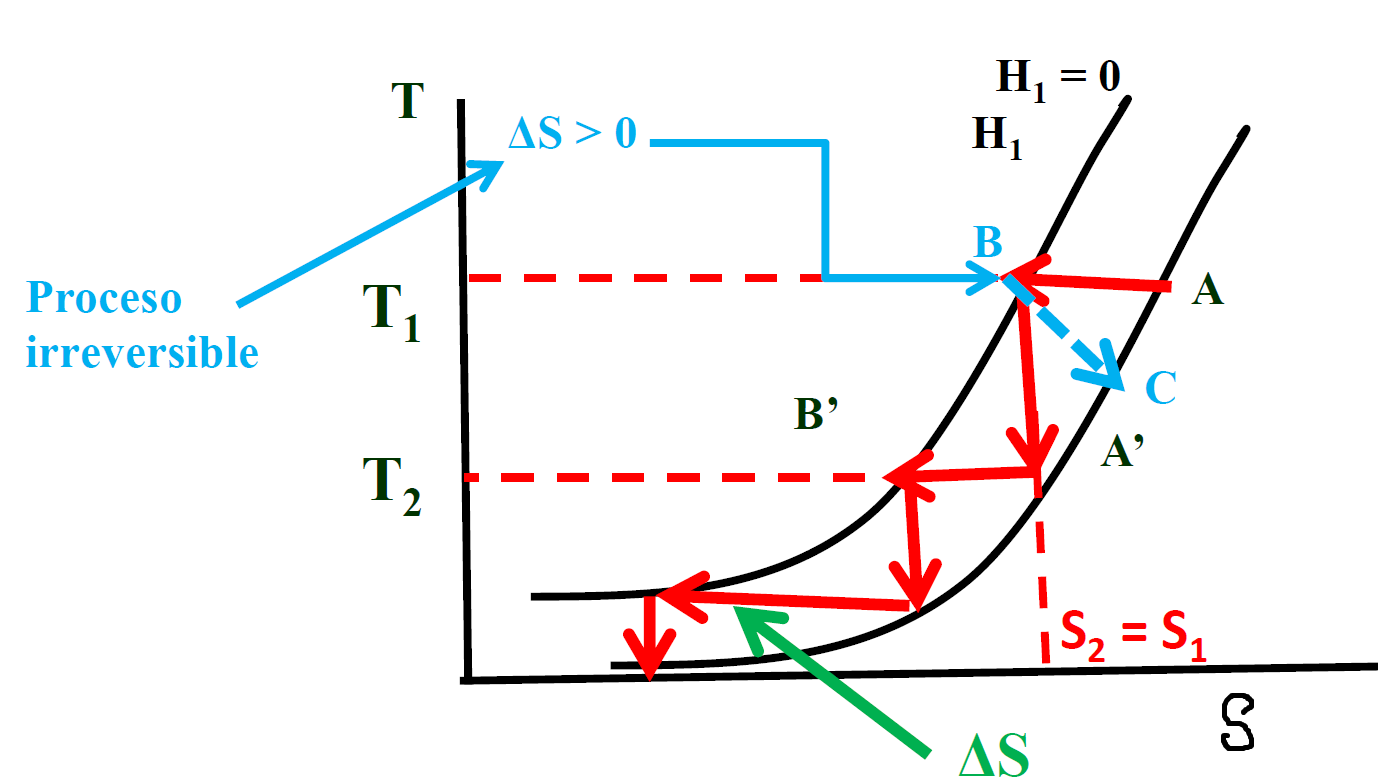
\includegraphics[scale=0.5]{Ceroabsoluto.png}
\caption{esquema de procesos para llegar al $T=0K$}
\end{figure}

Aunque en un principio pueda parecer que haciendo esos procesos se puede llegar a $T=0K$, como la variación de entropía tiende a hacerse 0 cuando $T\longrightarrow0$ tenemos que poco a poco los tramos horizontales de los procesos van siendo cada vez mas y as pequeños  y que en el cero absoluto las dos curvas convergen al mismo valor de $S_0$ para $T=0K$. Sin embargo para llegar a este proceso necesitaríamos un número infinito de procesos, ya que cada vez las curvas se aproximan y en un límite finito no alcanzaríamos el 0. Si consideramos ya procesos irreversibles la inaccersibilidad es todavía superior. \\

Aunque Nerst afirma que para un sistema monocomponente la entropía en el cero absoluto es $S_0$, pero que puede ser diferente para otro sistema monocompontente. El enunciado de Plack asigna a esa constante el valor universal (para cualquier sistema)  de $S_0 = 0$. Esta justificación se basa en la mecánica estadística cuántica, que nos dice que cualquier sistema a temperatura nula se encuentra en su estado fundamental, que se supone único. \\

Este será nuestro tercer principio de la termodinámica: \\

\Teorema{\textbf{\underline{Tercer principio de la termodinámica:}} para substancias puras, cristalinas y perfectamente ordenadas su entropía en el cero absoluto es nula, mientras que para todas las demás especies químicas es positiva: $$ \lim_{T \rightarrow 0} S = 0 $$} \\

Las consecuencias de este enunciado: 

\begin{itemize}
\item Identifica la isoterma $T=0$ con la adiabática $S=0$, aunque las otras isotermas y adiabáticas sean diferentes.

\item Que la entropía de cualquier sistema sea 0 en el cero absoluto es una contante universal.

\item En enunciado de Planck conduce al de Nerst, el de Nerst no conduce al de Planck
\end{itemize}
\newpage
\appendix 

\section{Anexo}
\subsection{Trabajos termodinámicos}

\begin{itemize}

\item \textbf{Trabajo en un fluido:} en este caso la magnitud intensiva es la presión (p) y la magnitud extensiva el volumen. El trabajo viene dado por:

\begin{equation}
\D ' W = - p \D V
\end{equation}

Se define así, con un signo negativo, ya que la presión es ejercida siempre por el pistón, y el volumen aumenta cuando el pistón va en dirección contraria a la presión. Entonces cuando esto ocurre el trabajo debe ser negativo (ya que tienen diferentes direcciones las magnitudes). Para que el trabajo sea negativo debe haber un menos que indique esta no mutua direccionalidad, y que la presión sea positiva. 

\item \textbf{Trabajo al  variar la longitud de un alambre:} en este caso la magnitud intensiva será la fuerza que aplicamos y la magnitud extensiva es la longitud del alambre (barilla, palo...) que será L. Entonces el trabajo viene dado por:

\begin{equation}
\D W' = F \D L
\end{equation}

En muchos ejercicios nos dan el módulo de Young del alambre. Para un alambre de sección A tenemos que el módulo de young por la sección se comporta igual que k (constante recuperación muelle):

\begin{equation}
\Delta F = k \dfrac{\Delta L}{L} = Y A \dfrac{\Delta L}{L} \Longrightarrow \parentesis{\dfrac{\D F}{\D L}}= \dfrac{Y A}{L}
\end{equation}

\item \textbf{Trabajo al variar el área de una superficie:} la variable intensiva será la tensión superficial ($\sigma$) que vendrá dada por las interacciones de las moléculas de la superficie en cuestión y la variable extensiva será la superficie (S):

\begin{equation}
\D ' W = 2 \sigma \D S
\end{equation}

Aparece un dos porque las superficies casi siempre una superficie presenta dos caras. 

\item \textbf{Trabajo al variar la carga:} la variable intensiva es la fuerza electromotriz o potencial eléctrico ($\epsilon$, $V$) y la extensiva la carga:

\begin{equation}
\D' W = \epsilon \D Q
\end{equation}

En los ejercicios a veces no nos dan cual es la diferencia de carga, pero si nos dicen que se aplica una intensidad constante en un determinado tiempo finito. En ese caso hay que saber que:

$$ \D  Q =  I \D t $$

La fuerza electromotriz se mide en voltios y la carga en coulombios.

\item \textbf{Trabajo al variar la imanación de un sólido magnético:}  en este caso la variable intensiva es la intensidad magnética H y la variable extensiva M, que es el momento magnético total. 

\begin{equation}
\D ' W = H \D M
\end{equation}

\item \textbf{Trabajo al variar la polarización de un sólido dieléctrico:} la variable intensiva será  el campo eléctrico E y la variable intensiva el momento dipolar total del dieléctrico $\Pi$. 

\begin{equation}
\D W' = E \D \Pi
\end{equation}

\end{itemize}



\subsection{Ecuaciones de gases}

\begin{itemize}
\item \textbf{Gases ideales:} 

\begin{equation}
 P V = n R T 
\end{equation}

\item  \textbf{Gas de van der Walls:} 
\begin{equation}
\parentesis{P + \dfrac{a}{V}}(V-b)=RT
\end{equation}
\end{itemize}


\subsection{Punto triple \label{Sub:anex-punto-triple}}

Llamamos punto triple al punto donde se pueden encontrar los 3 estados de la materia (gas, líquido, sólido) en equilibrio termodinámico. Ocurre con condiciones muy específicas, y una simple variación de las coordenadas termodinámicas hace que el equilbrio se modifique. En el caso del agua ocurre cuando T=273,16 K y p=0.0060 atm: \\

\begin{figure}[h!] \centering
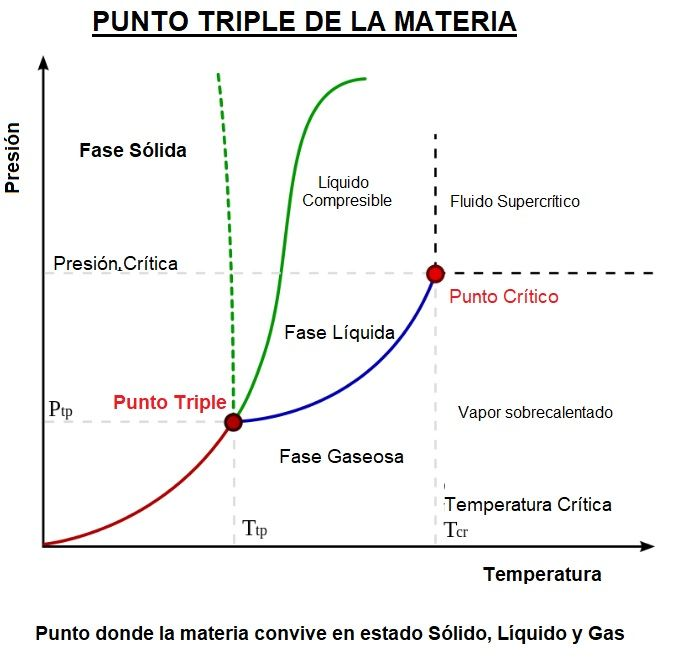
\includegraphics[scale=0.4]{Punto-triple-agua.png}
\end{figure}


\subsection{Homogénea de grado n \label{sub:anex-homogenea}}
Si una ecuación $F=F(x_1,x_2,\ldots, x_r, x'_1, x'_2, \ldots, x'_s)$ es homogénea de grado n en $x_1, x_2, \ldots, x_r$ entonces tenemos que:

\begin{equation}
\sum_{i=1}^r  \parentesis{\parciales{F}{x_i}}_{j \neq i} x_i = n F
\end{equation}

\end{document}

